%2multibyte Version: 5.50.0.2960 CodePage: 65001
% !TeX root = ./Slides_Lez_06_Processi_Stocastici_Tempo_Continuo.tex
%TCIDATA{OutputFilter=latex2.dll}
%TCIDATA{Version=5.50.0.2960}
%TCIDATA{Codepage=65001}
%TCIDATA{CSTFile=beamer.cst}
%TCIDATA{Created=Sunday, June 14, 2026 10:00:00}
%TCIDATA{LastRevised=Sunday, June 14, 2026 10:00:00}
%TCIDATA{<META NAME="GraphicsSave" CONTENT="32">}
%TCIDATA{<META NAME="SaveForMode" CONTENT="2">}
%TCIDATA{BibliographyScheme=Manual}
%TCIDATA{<META NAME="DocumentShell" CONTENT="Other Documents\SW\Slides - Beamer">}
%BeginMSIPreambleData
\providecommand{\U}[1]{\protect\rule{.1in}{.1in}}
%EndMSIPreambleData

\documentclass[handout]{beamer}
\usepackage{mathpazo}
\usepackage{multimedia}
\usepackage{amsmath}
\usepackage{amsfonts}
\usepackage{amssymb}
\usepackage{graphicx}
\setcounter{MaxMatrixCols}{30}

\newenvironment{stepenumerate}{\begin{enumerate}[<+->]}{\end{enumerate}}
\newenvironment{stepitemize}{\begin{itemize}[<+->]}{\end{itemize}}
\newenvironment{stepenumeratewithalert}{\begin{enumerate}[<+-| alert@+>]}{\end{enumerate}}
\newenvironment{stepitemizewithalert}{\begin{itemize}[<+-| alert@+>]}{\end{itemize}}
\usetheme{Madrid}

\setbeamertemplate{footline}
{
  \leavevmode%
  \hbox{%
    \begin{beamercolorbox}[wd=.20\paperwidth,ht=2.25ex,dp=1ex,center]
      {author in head/foot}%
      \usebeamerfont{author in head/foot}\insertshortauthor
    \end{beamercolorbox}%
    \begin{beamercolorbox}[wd=.69\paperwidth,ht=2.25ex,dp=1ex,center]
      {title in head/foot}%
      \usebeamerfont{title in head/foot}\insertshorttitle
    \end{beamercolorbox}%
    \begin{beamercolorbox}[wd=.11\paperwidth,ht=2.25ex,dp=1ex,right]
      {date in head/foot}%
      \usebeamerfont{date in head/foot}%
      \insertshortdate{}\hspace*{2em}%
      \insertframenumber{} / \inserttotalframenumber\hspace*{2ex}
    \end{beamercolorbox}%
  }%
  \vskip0pt%
}
\definecolor{light-blue}{rgb}{0.50,0.55,1.00}% 
\setbeamercolor{alerted text}{fg=light-blue}
\providecommand{\R}{\mathbb{R}}
\providecommand{\N}{\mathbb{N}}
\providecommand{\E}{\mathbb{E}}
\providecommand{\Prob}{\mathbb{P}}
\providecommand{\Q}{\mathbb{Q}}
\providecommand{\F}{\mathcal{F}}
\providecommand{\B}{\mathcal{B}}
\providecommand{\G}{\mathcal{G}}
\providecommand{\Corr}{\operatorname{Corr}}
\providecommand{\Var}{\operatorname{Var}}
\providecommand{\Cov}{\operatorname{Cov}}
\providecommand{\VaR}{\operatorname{VaR}}
\providecommand{\CVaR}{\operatorname{CVaR}}
\providecommand{\argmin}{\operatorname*{arg\,min}}
\providecommand{\argmax}{\operatorname*{arg\,max}}
\providecommand{\EVPI}{\operatorname{EVPI}}
\providecommand{\VSS}{\operatorname{VSS}}
\providecommand{\QTR}[2]{\csname #1\endcsname{#2}}

\title[Lez. 6 - Processi stocastici II -- Tempo continuo: diffusioni,
mean-reversion e simulazione]{Lezione 6 - Processi stocastici II -- Tempo continuo: diffusioni,
mean-reversion e simulazione}
\subtitle{Metodi Quantitativi per la Finanza}
\author[P. Falbo, C. Pelizzari]{{\LARGE Paolo Falbo, Cristian Pelizzari}}
\institute[]{{\large Dipartimento di Economia e Management}}
\date[]{}
\titlegraphic{

\includegraphics[height=1.25cm]{../graphics/MQF_logo.png}\hspace{0.8cm}%

\includegraphics[height=1.25cm]{../graphics/logo-Unibs-esteso.png}}

\begin{document}
\maketitle

%********************
% GRUPPO 1 - APERTURA E ORIENTAMENTO
% Slide 1-3
% Tempo parziale: 7 minuti | Tempo cumulato: 7 minuti
%********************

\section{Apertura}

% Slide 1 - Domanda guida

\subsection{Domanda guida}

%TCIMACRO{\TeXButton{BeginFrame}{\begin{frame}}}%
%BeginExpansion
\begin{frame}%
%EndExpansion

\QTR{frametitle}{La domanda guida: traiettorie in tempo continuo}

%TCIMACRO{\TeXButton{Transparency}{\setbeamercovered{transparent=20}}}%
%BeginExpansion
\setbeamercovered{transparent=20}%
%EndExpansion

\begin{center}
{\large Come si modellano fattori finanziari che evolvono con continuit\`a
nel tempo, e come si preparano alla simulazione?}
\end{center}

\medskip

Nella Lezione 5 abbiamo costruito il linguaggio dei processi stocastici:
\[
\text{traiettorie}
\quad\text{--}\quad
\text{informazione}
\quad\text{--}\quad
\text{martingale}.
\]
Ora l'indice temporale varia con continuit\`a: $\{X_t\}_{t\geq 0}$.

\medskip

Un modello in tempo continuo si costruisce con tre ingredienti:

\begin{stepitemize}
\item una sorgente di incertezza: gli \textbf{incrementi browniani};
\item una \textbf{dinamica locale} che d\`a forma a quell'incertezza:
drift e diffusione;
\item una \textbf{griglia temporale} su cui generare le traiettorie.
\end{stepitemize}
%TCIMACRO{\TeXButton{Transition: Box Out}{\transboxout}}%
%BeginExpansion
\transboxout%
%EndExpansion
%TCIMACRO{\TeXButton{EndFrame}{\end{frame}}}%
%BeginExpansion
\end{frame}%
%EndExpansion
%*

% Slide 2 - Motivazione finanziaria: i due casi

\subsection{Due casi}

%TCIMACRO{\TeXButton{BeginFrame}{\begin{frame}}}%
%BeginExpansion
\begin{frame}%
%EndExpansion

\QTR{frametitle}{Due casi che chiedono intere traiettorie}

%TCIMACRO{\TeXButton{Transparency}{\setbeamercovered{transparent=20}}}%
%BeginExpansion
\setbeamercovered{transparent=20}%
%EndExpansion

\begin{stepitemize}

\item \textbf{Caso A.} Una banca deve valutare un contratto su un titolo
il cui payoff dipende dai livelli raggiunti durante la vita del
contratto, per esempio dalla media dei prezzi.

Fattore da modellare: il prezzo $S_t$.

\medskip

\item \textbf{Caso B.} Un fondo pensione deve valutare un'obbligazione i
cui flussi sono indicizzati all'inflazione e il cui valore attuale
dipende dall'evoluzione dei tassi di interesse.

Fattori da modellare: l'inflazione e il tasso istantaneo $r_t$, che
evolvono insieme.

\end{stepitemize}

\medskip

In entrambi i casi non basta la distribuzione di una variabile
terminale: occorre l'evoluzione delle grandezze rilevanti lungo l'intero
orizzonte.

\medskip

\begin{center}
{\large Come si descrivono e si generano queste traiettorie?}
\end{center}
%TCIMACRO{\TeXButton{Transition: Box Out}{\transboxout}}%
%BeginExpansion
\transboxout%
%EndExpansion
%TCIMACRO{\TeXButton{EndFrame}{\end{frame}}}%
%BeginExpansion
\end{frame}%
%EndExpansion
%*

% Slide 3 - Mappa del percorso

\subsection{Percorso della lezione}

%TCIMACRO{\TeXButton{BeginFrame}{\begin{frame}}}%
%BeginExpansion
\begin{frame}%
%EndExpansion

\QTR{frametitle}{Il percorso: ogni passo nasce dal limite del precedente}

%TCIMACRO{\TeXButton{Transparency}{\setbeamercovered{transparent=20}}}%
%BeginExpansion
\setbeamercovered{transparent=20}%
%EndExpansion

{\scriptsize
\renewcommand{\arraystretch}{1.3}
\begin{center}
\begin{tabular}{|c|p{1.9cm}|p{4.9cm}|p{2.7cm}|}
\hline
\textbf{Passo} & \textbf{Tema} & \textbf{Domanda} & \textbf{Strumento} \\
\hline
1 & Il rumore & Quanto \`e grande uno shock su $\Delta t$? & $W_t$, scala $\sqrt{\Delta t}$ \\
\hline
2 & La forma & Quali propriet\`a deve avere il processo? & SDE: GBM, OU, CIR \\
\hline
3 & La dipendenza & I processi si muovono insieme? & shock correlati \\
\hline
4 & La simulazione & Come si genera la traiettoria? & Eulero-Maruyama \\
\hline
\end{tabular}
\end{center}
}

\begin{stepitemize}
\item Il rumore browniano fornisce lo shock, ma non le propriet\`a
economiche.
\item Drift e diffusione danno forma al rumore: un modello per ciascun
caso.
\item Nel Caso B gli shock non sono indipendenti: vanno
costruiti congiuntamente.
\item La dinamica continua viene riportata su una griglia e diventa
traiettoria simulata.
\end{stepitemize}
%TCIMACRO{\TeXButton{Transition: Box Out}{\transboxout}}%
%BeginExpansion
\transboxout%
%EndExpansion
%TCIMACRO{\TeXButton{EndFrame}{\end{frame}}}%
%BeginExpansion
\end{frame}%
%EndExpansion
%*

%********************
% GRUPPO 2 - PASSO 1: IL RUMORE (MOTO BROWNIANO)
% Divisorio + Slide 4-8
% Tempo parziale: 12 minuti | Tempo cumulato: 19 minuti
%********************

\section{\texorpdfstring{Passo 1 -- Il rumore}{Passo 1 - Il rumore}}

%TCIMACRO{\TeXButton{BeginFrame}{\begin{frame}}}%
%BeginExpansion
\begin{frame}%
%EndExpansion

\setbeamertemplate{headline}{}

\vfill

\begin{center}
\textcolor{light-blue}{{\Large \textbf{Passo 1 -- Il rumore: il moto browniano}}}
\end{center}

\vfill

{\scriptsize
\renewcommand{\arraystretch}{1.3}
\begin{center}
\begin{tabular}{|c|p{1.9cm}|p{4.9cm}|p{2.7cm}|}
\hline
\textbf{Passo} & \textbf{Tema} & \textbf{Domanda} & \textbf{Strumento} \\
\hline
\leavevmode\alert{1} & \leavevmode\alert{Il rumore} & \leavevmode\alert{Quanto \`e grande uno shock su $\Delta t$?} & \leavevmode\alert{$W_t$, scala $\sqrt{\Delta t}$} \\
\hline
2 & La forma & Quali propriet\`a deve avere il fattore? & SDE: GBM, OU, CIR \\
\hline
3 & La dipendenza & I fattori si muovono insieme? & shock correlati \\
\hline
4 & La simulazione & Come si genera la traiettoria? & Eulero-Maruyama \\
\hline
\end{tabular}
\end{center}
}

\vfill

%TCIMACRO{\TeXButton{Transition: Box Out}{\transboxout}}%
%BeginExpansion
\transboxout%
%EndExpansion
%TCIMACRO{\TeXButton{EndFrame}{\end{frame}}}%
%BeginExpansion
\end{frame}%
%EndExpansion
%*

% Slide 4 - Passeggiata aleatoria riscalata

\subsection{Passeggiata aleatoria riscalata}

%TCIMACRO{\TeXButton{BeginFrame}{\begin{frame}}}%
%BeginExpansion
\begin{frame}%
%EndExpansion

\QTR{frametitle}{Si parte da una griglia: la passeggiata aleatoria riscalata}

%TCIMACRO{\TeXButton{Transparency}{\setbeamercovered{transparent=20}}}%
%BeginExpansion
\setbeamercovered{transparent=20}%
%EndExpansion

\textcolor{light-blue}{Il modo pi\`u semplice di generare incertezza nel tempo: sommare shock indipendenti su una griglia.}

\medskip

Consideriamo una griglia uniforme dell'intervallo $[0,T]$:
\[
0=t_0<t_1<\cdots<t_n=T,
\qquad
\Delta t=\frac{T}{n}.
\]
A ogni intervallo associamo una innovazione gaussiana indipendente
\[
Z_1,\ldots,Z_n\sim\mathcal{N}(0,1).
\]
La passeggiata aleatoria riscalata \`e
\[
W_{t_j}^{(n)}
=
\sum_{k=1}^{j}\sqrt{\Delta t}\,Z_k,
\qquad
j=1,\ldots,n,
\]
e il singolo incremento sulla griglia \`e
\[
W_{t_j}^{(n)}-W_{t_{j-1}}^{(n)}
=
\sqrt{\Delta t}\,Z_j.
\]
%TCIMACRO{\TeXButton{Transition: Box Out}{\transboxout}}%
%BeginExpansion
\transboxout%
%EndExpansion
%TCIMACRO{\TeXButton{EndFrame}{\end{frame}}}%
%BeginExpansion
\end{frame}%
%EndExpansion
%*

% Slide 5 - Raffinamento della griglia e ripresa della Lezione 5

\subsection{Raffinamento della griglia}

%TCIMACRO{\TeXButton{BeginFrame}{\begin{frame}}}%
%BeginExpansion
\begin{frame}%
%EndExpansion

\QTR{frametitle}{Raffinando la griglia, la struttura della varianza non cambia}

%TCIMACRO{\TeXButton{Transparency}{\setbeamercovered{transparent=20}}}%
%BeginExpansion
\setbeamercovered{transparent=20}%
%EndExpansion

Per ogni incremento della passeggiata riscalata:
\[
\E\left[W_{t_j}^{(n)}-W_{t_{j-1}}^{(n)}\right]=0,
\qquad
\Var\left(W_{t_j}^{(n)}-W_{t_{j-1}}^{(n)}\right)=\Delta t.
\]

\begin{stepitemize}

\item Raffinando la griglia, $\Delta t$ diminuisce e i singoli
incrementi diventano pi\`u piccoli, ma la varianza accumulata su
$[0,T]$ resta $n\Delta t=T$.

\item La covarianza fra due tempi della griglia \`e
\[
\Cov\left(W_{t_i}^{(n)},W_{t_j}^{(n)}\right)=\min(t_i,t_j):
\]
\`e la struttura $\min(s,t)\,\tau^2$ della passeggiata aleatoria della
Lezione 5, con varianza per unit\`a di tempo pari a $1$.

\item Nel passaggio al tempo continuo si conserva proprio questa
struttura: incrementi indipendenti con varianza pari alla durata
dell'intervallo.

\end{stepitemize}
%TCIMACRO{\TeXButton{Transition: Box Out}{\transboxout}}%
%BeginExpansion
\transboxout%
%EndExpansion
%TCIMACRO{\TeXButton{EndFrame}{\end{frame}}}%
%BeginExpansion
\end{frame}%
%EndExpansion
%*

% Slide 6 - Moto browniano standard

\subsection{Moto browniano standard}

%TCIMACRO{\TeXButton{BeginFrame}{\begin{frame}}}%
%BeginExpansion
\begin{frame}%
%EndExpansion

\QTR{frametitle}{Il limite della griglia: il moto browniano standard}

%TCIMACRO{\TeXButton{Transparency}{\setbeamercovered{transparent=20}}}%
%BeginExpansion
\setbeamercovered{transparent=20}%
%EndExpansion

Un processo $\{W_t\}_{t\geq0}$ \`e un \textbf{moto browniano
standard} se:

\begin{stepenumerate}

\item[1.] parte dall'origine: $W_0=0$;

\item[2.] le traiettorie $t\mapsto W_t(\omega)$ sono continue;

\item[3.] gli incrementi su intervalli temporali disgiunti sono
indipendenti;

\item[4.] per ogni intervallo $0\leq s<t$,
\[
W_t-W_s
\sim
\mathcal{N}(0,t-s).
\]

\end{stepenumerate}

\medskip

Ne seguono
\[
\E[W_t]=0,
\qquad
\Var(W_t)=t,
\qquad
\Cov(W_s,W_t)=\min(s,t).
\]

La distribuzione dell'incremento dipende dalla lunghezza
dell'intervallo, non dalla sua posizione nel tempo.
%TCIMACRO{\TeXButton{Transition: Box Out}{\transboxout}}%
%BeginExpansion
\transboxout%
%EndExpansion
%TCIMACRO{\TeXButton{EndFrame}{\end{frame}}}%
%BeginExpansion
\end{frame}%
%EndExpansion
%*

% Slide 7 - Scala degli incrementi

\subsection{Scala degli incrementi}

%TCIMACRO{\TeXButton{BeginFrame}{\begin{frame}}}%
%BeginExpansion
\begin{frame}%
%EndExpansion

\QTR{frametitle}{Lo shock su $\Delta t$ scala con $\sqrt{\Delta t}$, non con $\Delta t$}

%TCIMACRO{\TeXButton{Transparency}{\setbeamercovered{transparent=20}}}%
%BeginExpansion
\setbeamercovered{transparent=20}%
%EndExpansion

Su un intervallo di ampiezza $\Delta t$,
\[
\Delta W_t
=
W_{t+\Delta t}-W_t
\sim
\mathcal{N}(0,\Delta t).
\]
Quindi
\[
\E[\Delta W_t]=0,
\qquad
\Var(\Delta W_t)=\Delta t,
\qquad
\operatorname{sd}(\Delta W_t)=\sqrt{\Delta t}.
\]
Per simulare l'incremento si usa
\[
\Delta W_t
=
\sqrt{\Delta t}\,Z,
\qquad
Z\sim\mathcal{N}(0,1).
\]

\begin{stepitemize}
\item $Z$ \`e una innovazione standardizzata.
\item $\Delta W_t$ \`e l'incremento browniano sull'intervallo effettivo.
\item Su intervalli brevi, $\sqrt{\Delta t}$ \`e molto pi\`u grande di
$\Delta t$: lo shock domina la variazione locale.
\end{stepitemize}
%TCIMACRO{\TeXButton{Transition: Box Out}{\transboxout}}%
%BeginExpansion
\transboxout%
%EndExpansion
%TCIMACRO{\TeXButton{EndFrame}{\end{frame}}}%
%BeginExpansion
\end{frame}%
%EndExpansion
%*

% Slide 8 - Traiettorie browniane e ponte

\subsection{Traiettorie browniane}

%TCIMACRO{\TeXButton{BeginFrame}{\begin{frame}}}%
%BeginExpansion
\begin{frame}%
%EndExpansion

\QTR{frametitle}{Traiettorie continue, irregolari, sempre pi\`u disperse}

%TCIMACRO{\TeXButton{Transparency}{\setbeamercovered{transparent=20}}}%
%BeginExpansion
\setbeamercovered{transparent=20}%
%EndExpansion

\begin{center}
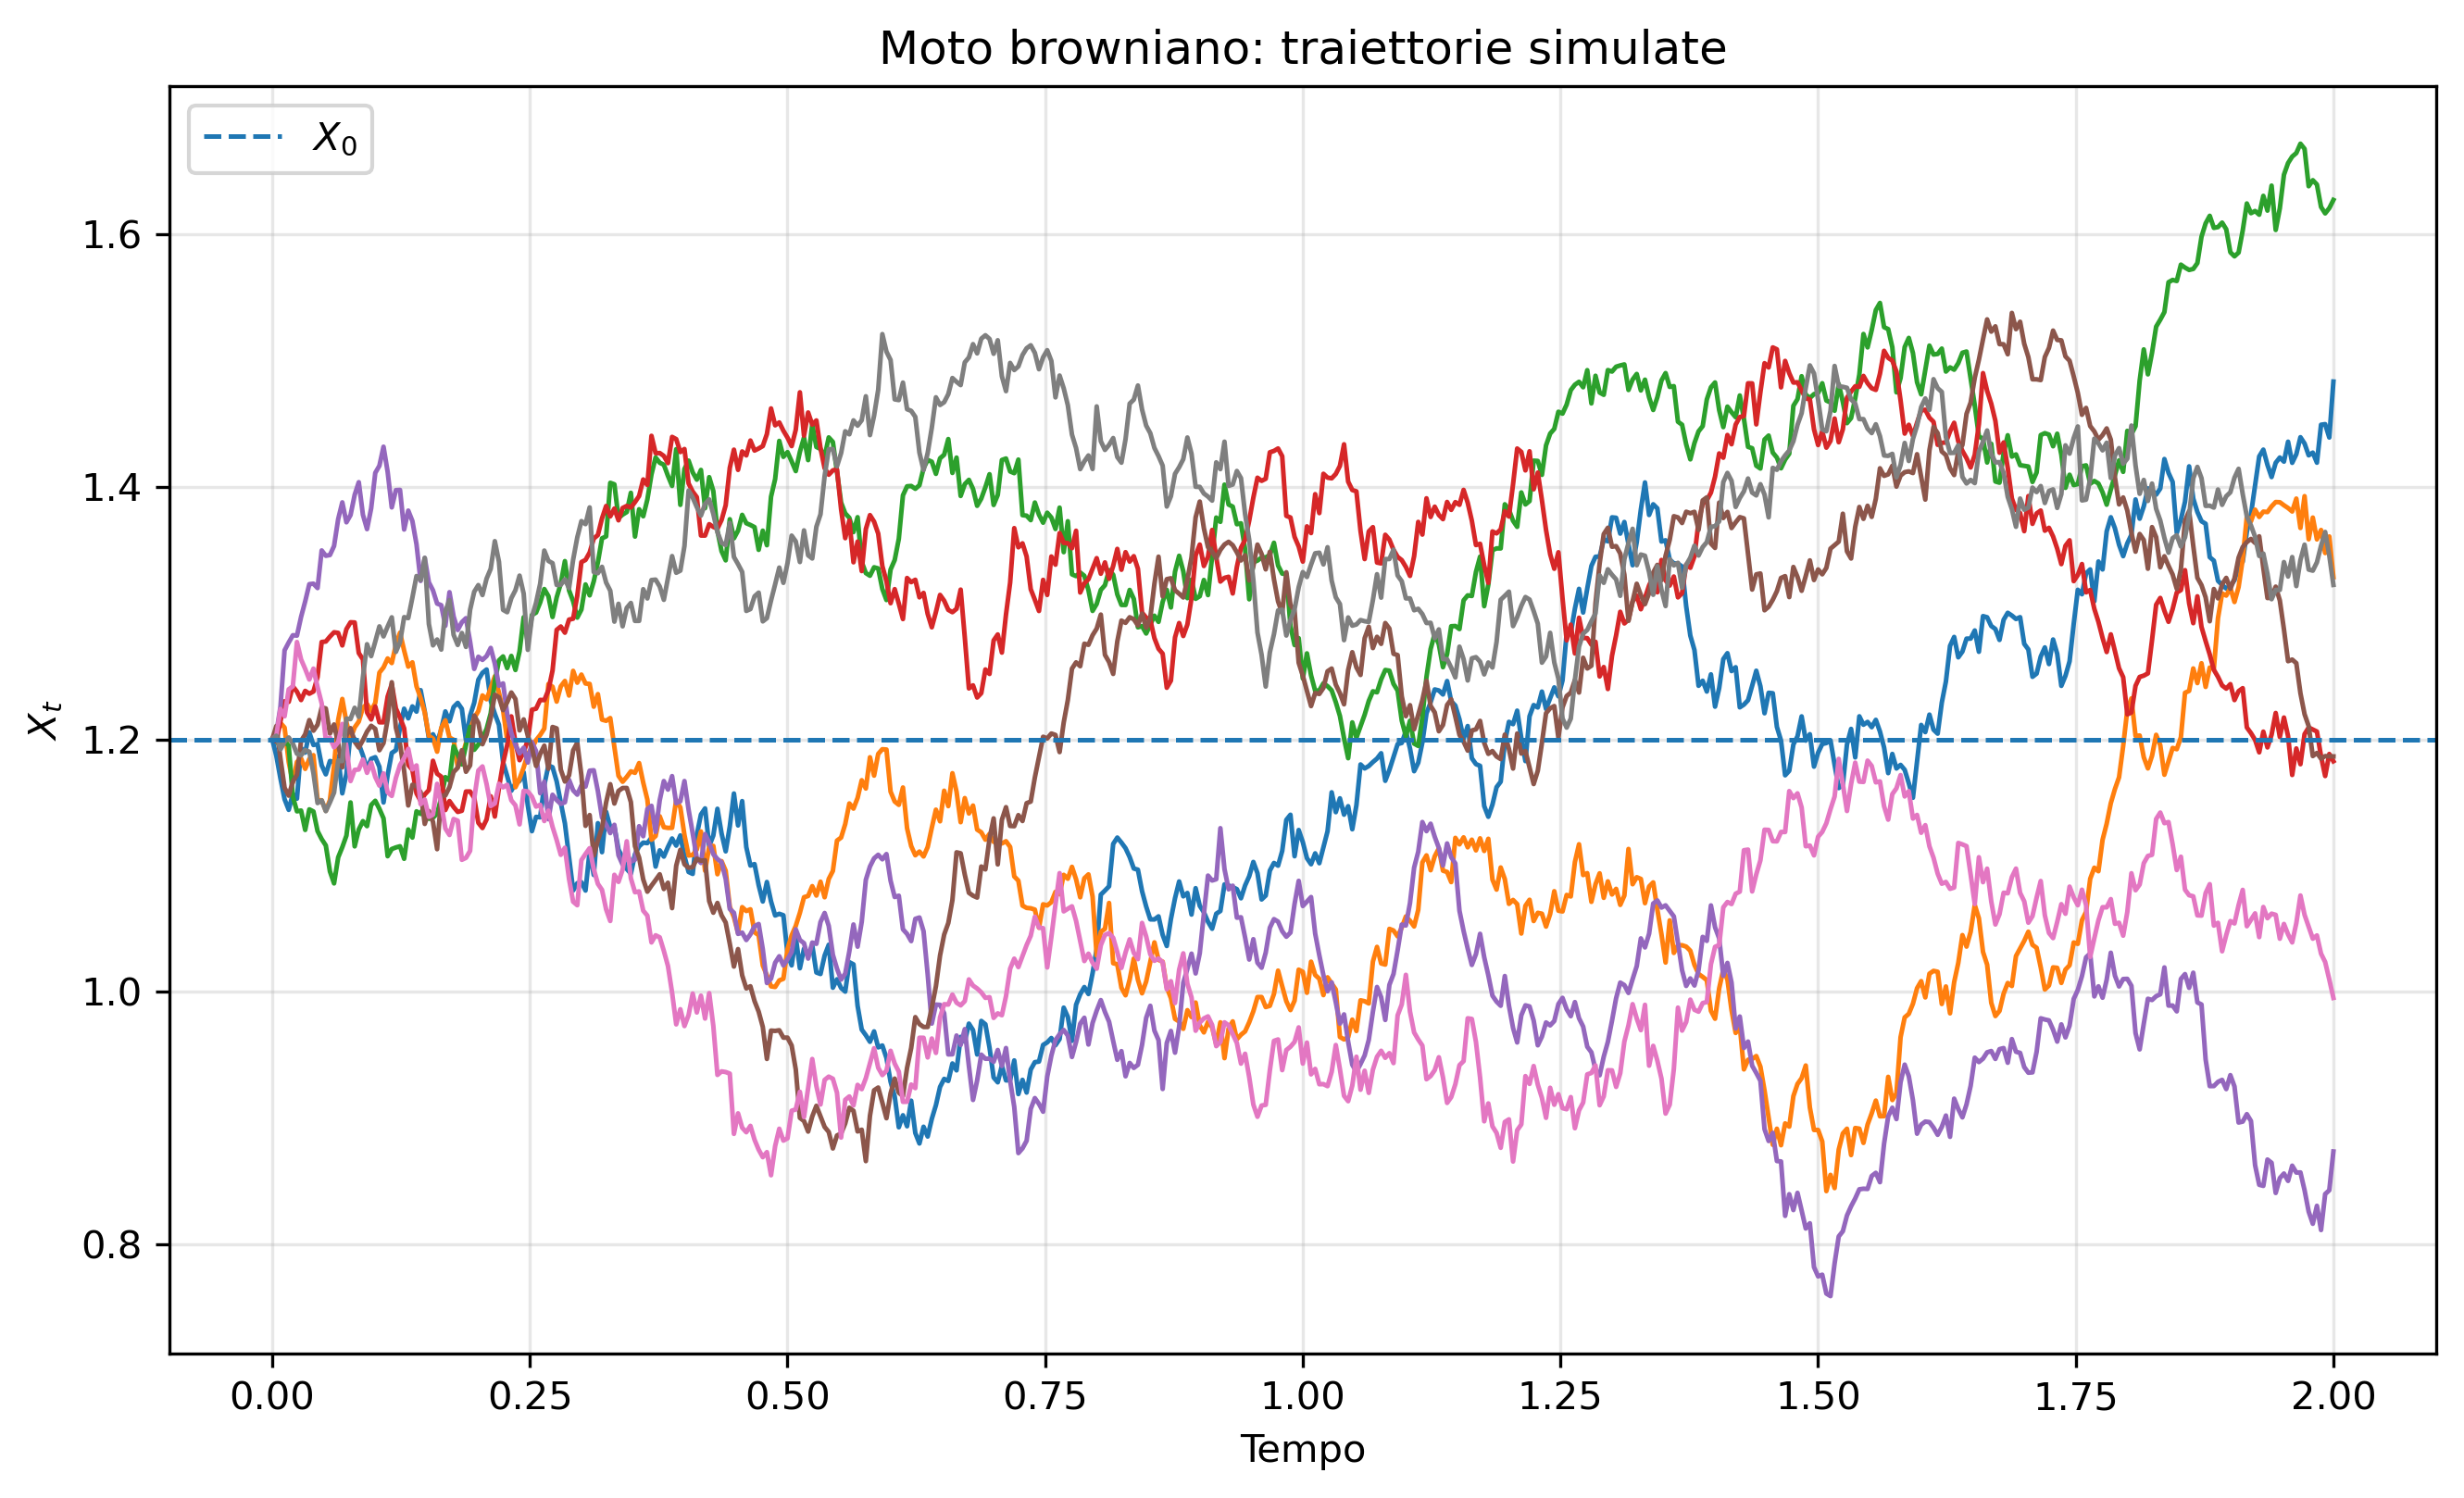
\includegraphics[width=0.6\textwidth]
{../graphics/Cap06_Brownian_traiettorie.png}
\end{center}

\begin{stepitemize}

\item Le traiettorie sono continue, ma irregolari.

\item La dispersione aumenta con l'orizzonte temporale, poich\'e
$\Var(W_t)=t$.

\item \textcolor{light-blue}{Il moto browniano \`e la materia prima degli
shock, ma non ha forma: non resta positivo e non torna verso alcun
livello. Prima di dargli forma, una conseguenza immediata per il rischio.}

\end{stepitemize}
%TCIMACRO{\TeXButton{Transition: Box Out}{\transboxout}}%
%BeginExpansion
\transboxout%
%EndExpansion
%TCIMACRO{\TeXButton{EndFrame}{\end{frame}}}%
%BeginExpansion
\end{frame}%
%EndExpansion
%*

%********************
% GRUPPO 3 - ESERCIZIO IN AULA: SCALA TEMPORALE DEL RISCHIO
% Slide 9-11
% Tempo parziale: 8 minuti | Tempo cumulato: 27 minuti
%********************

% Slide 9 - Esercizio

\subsection{Esercizio: scala temporale del rischio}

%TCIMACRO{\TeXButton{BeginFrame}{\begin{frame}}}%
%BeginExpansion
\begin{frame}%
%EndExpansion

\QTR{frametitle}{Esercizio: dal rischio giornaliero al rischio su cinque giorni}

%TCIMACRO{\TeXButton{Transparency}{\setbeamercovered{transparent=20}}}%
%BeginExpansion
\setbeamercovered{transparent=20}%
%EndExpansion

La componente aleatoria del rendimento di un'attivit\`a su un
orizzonte $h$ \`e
\[
R_h
=
\sigma\left(W_{t+h}-W_t\right),
\]
con volatilit\`a annualizzata
\[
\sigma=0.20.
\]
Si assumano $252$ giorni di mercato in un anno.

\medskip

Determinare:

\begin{stepenumerate}

\item[1.] la deviazione standard dello shock giornaliero;

\item[2.] la deviazione standard dello shock su cinque giorni;

\item[3.] il rapporto tra le due deviazioni standard;

\item[4.] la probabilit\`a che lo shock giornaliero sia inferiore al
$-2\%$.

\end{stepenumerate}
%TCIMACRO{\TeXButton{Transition: Box Out}{\transboxout}}%
%BeginExpansion
\transboxout%
%EndExpansion
%TCIMACRO{\TeXButton{EndFrame}{\end{frame}}}%
%BeginExpansion
\end{frame}%
%EndExpansion
%*

% Slide 10 - Soluzione punti 1-3

\subsection{Regola della radice del tempo}

%TCIMACRO{\TeXButton{BeginFrame}{\begin{frame}}}%
%BeginExpansion
\begin{frame}%
%EndExpansion

\QTR{frametitle}{Soluzione: il rischio cresce con la radice dell'orizzonte}

%TCIMACRO{\TeXButton{Transparency}{\setbeamercovered{transparent=20}}}%
%BeginExpansion
\setbeamercovered{transparent=20}%
%EndExpansion

Poich\'e su un intervallo annuale $[0,h]$
\[
R_h\sim\mathcal{N}(0,\sigma^2h),
\qquad
\operatorname{sd}(R_h)=\sigma\sqrt{h},
\]
per un intervallo giornaliero si ottiene:

{\small
\[
\operatorname{sd}(R_{1/252})
=
0.20\sqrt{\frac{1}{252}}
\approx0.0126,
\qquad
\operatorname{sd}(R_{5/252})
=
0.20\sqrt{\frac{5}{252}}
\approx0.0282.
\]
}

Pertanto,
\[
\frac{\operatorname{sd}(R_{5/252})}
{\operatorname{sd}(R_{1/252})}
=
\sqrt{5}
\approx
2.236.
\]

Quintuplicare l'orizzonte non quintuplica il rischio: la deviazione
standard a cinque giorni \`e circa $2.24$ volte quella giornaliera.
%TCIMACRO{\TeXButton{Transition: Box Out}{\transboxout}}%
%BeginExpansion
\transboxout%
%EndExpansion
%TCIMACRO{\TeXButton{EndFrame}{\end{frame}}}%
%BeginExpansion
\end{frame}%
%EndExpansion
%*

% Slide 11 - Soluzione punto 4 e ponte al passo 2

\subsection{Probabilit\`a di coda}

%TCIMACRO{\TeXButton{BeginFrame}{\begin{frame}}}%
%BeginExpansion
\begin{frame}%
%EndExpansion

\QTR{frametitle}{Soluzione: uno shock giornaliero sotto il $-2\%$}

%TCIMACRO{\TeXButton{Transparency}{\setbeamercovered{transparent=20}}}%
%BeginExpansion
\setbeamercovered{transparent=20}%
%EndExpansion

Lo shock giornaliero soddisfa
\[
R_{1/252}
\sim
\mathcal{N}
\left(
0,
\frac{0.20^2}{252}
\right),
\qquad
\operatorname{sd}(R_{1/252})
\approx
0.0126.
\]
Standardizzando,
\[
\Prob(R_{1/252}<-0.02)
=
\Phi
\left(
\frac{-0.02}{0.0126}
\right)
=
\Phi(-1.587)
\approx
0.0562.
\]
La probabilit\`a richiesta \`e quindi circa il $5.6\%$.

\bigskip

\textcolor{light-blue}{Per modellare altri oggetti finanziari (prezzi, tassi interesse, di inflazione,...) il moto browniano non è sufficientemente articolato.}
%TCIMACRO{\TeXButton{Transition: Box Out}{\transboxout}}%
%BeginExpansion
\transboxout%
%EndExpansion
%TCIMACRO{\TeXButton{EndFrame}{\end{frame}}}%
%BeginExpansion
\end{frame}%
%EndExpansion
%*

%********************
% GRUPPO 4 - PASSO 2: LA FORMA (EQUAZIONI DIFFERENZIALI STOCASTICHE)
% Divisorio + Slide 12-14
% Tempo parziale: 10 minuti | Tempo cumulato: 37 minuti
%********************

\section{\texorpdfstring{Passo 2 -- La forma}{Passo 2 - La forma}}

%TCIMACRO{\TeXButton{BeginFrame}{\begin{frame}}}%
%BeginExpansion
\begin{frame}%
%EndExpansion

\setbeamertemplate{headline}{}

\vfill

\begin{center}
\textcolor{light-blue}{{\Large \textbf{Passo 2 -- La forma: drift e diffusione}}}
\end{center}

\vfill

{\scriptsize
\renewcommand{\arraystretch}{1.3}
\begin{center}
\begin{tabular}{|c|p{1.9cm}|p{4.9cm}|p{2.7cm}|}
\hline
\textbf{Passo} & \textbf{Tema} & \textbf{Domanda} & \textbf{Strumento} \\
\hline
1 & Il rumore & Quanto \`e grande uno shock su $\Delta t$? & $W_t$, scala $\sqrt{\Delta t}$ \\
\hline
\leavevmode\alert{2} & \leavevmode\alert{La forma} & \leavevmode\alert{Quali propriet\`a deve avere il fattore?} & \leavevmode\alert{SDE: GBM, OU, CIR} \\
\hline
3 & La dipendenza & I fattori si muovono insieme? & shock correlati \\
\hline
4 & La simulazione & Come si genera la traiettoria? & Eulero-Maruyama \\
\hline
\end{tabular}
\end{center}
}

\vfill

%TCIMACRO{\TeXButton{Transition: Box Out}{\transboxout}}%
%BeginExpansion
\transboxout%
%EndExpansion
%TCIMACRO{\TeXButton{EndFrame}{\end{frame}}}%
%BeginExpansion
\end{frame}%
%EndExpansion
%*

% Slide 12 - Struttura generale di una diffusione

\subsection{Struttura generale}

%TCIMACRO{\TeXButton{BeginFrame}{\begin{frame}}}%
%BeginExpansion
\begin{frame}%
%EndExpansion

\QTR{frametitle}{Una SDE d\`a forma al rumore: drift e diffusione}

%TCIMACRO{\TeXButton{Transparency}{\setbeamercovered{transparent=20}}}%
%BeginExpansion
\setbeamercovered{transparent=20}%
%EndExpansion

Una diffusione in tempo continuo \`e descritta da una \textbf{equazione differenziale stocastica}:
\[
dX_t
=
a(X_t,t)\,dt
+
b(X_t,t)\,dW_t.
\]

\begin{stepitemize}

\item Il coefficiente $a(X_t,t)$ determina il \textbf{drift}:
la componente sistematica della variazione.

\item Il coefficiente $b(X_t,t)$ determina la \textbf{diffusione}:
l'intensit\`a con cui lo shock browniano entra nella dinamica.

\item Entrambi i coefficienti possono dipendere dal
\textbf{livello corrente} $X_t$ e dal \textbf{tempo} $t$.

\end{stepitemize}

\medskip

Il simbolo $dW_t$ rappresenta un incremento browniano elementare:
non \`e un differenziale ordinario.
%TCIMACRO{\TeXButton{Transition: Box Out}{\transboxout}}%
%BeginExpansion
\transboxout%
%EndExpansion
%TCIMACRO{\TeXButton{EndFrame}{\end{frame}}}%
%BeginExpansion
\end{frame}%
%EndExpansion
%*

% Slide 13 - Drift e diffusione: interpretazione locale

\subsection{Interpretazione locale}

%TCIMACRO{\TeXButton{BeginFrame}{\begin{frame}}}%
%BeginExpansion
\begin{frame}%
%EndExpansion

\QTR{frametitle}{Il drift sposta la media, la diffusione scala lo shock}

%TCIMACRO{\TeXButton{Transparency}{\setbeamercovered{transparent=20}}}%
%BeginExpansion
\setbeamercovered{transparent=20}%
%EndExpansion

Su un intervallo temporale breve $\Delta t$,
\[
\Delta X_t
\approx
a(X_t,t)\,\Delta t
+
b(X_t,t)\sqrt{\Delta t}\,Z,
\qquad
Z\sim\mathcal{N}(0,1).
\]
Condizionatamente al livello corrente,
\[
\E[\Delta X_t\mid X_t]
\approx
a(X_t,t)\,\Delta t,
\qquad
\Var(\Delta X_t\mid X_t)
\approx
b^2(X_t,t)\,\Delta t.
\]

\begin{stepitemize}

\item Il \textbf{drift} governa la variazione media locale.

\item La \textbf{diffusione} governa la varianza locale.

\item La componente di drift \`e dell'ordine di $\Delta t$;
lo shock casuale \`e dell'ordine di $\sqrt{\Delta t}$, come nel passo 1.

\end{stepitemize}
%TCIMACRO{\TeXButton{Transition: Box Out}{\transboxout}}%
%BeginExpansion
\transboxout%
%EndExpansion
%TCIMACRO{\TeXButton{EndFrame}{\end{frame}}}%
%BeginExpansion
\end{frame}%
%EndExpansion
%*

% Slide 14 - Tre domande di progetto e scheda dei requisiti

\subsection{Tre domande di progetto}

%TCIMACRO{\TeXButton{BeginFrame}{\begin{frame}}}%
%BeginExpansion
\begin{frame}%
%EndExpansion

\QTR{frametitle}{Scegliere $a$ e $b$ significa scegliere le propriet\`a di un processo}

%TCIMACRO{\TeXButton{Transparency}{\setbeamercovered{transparent=20}}}%
%BeginExpansion
\setbeamercovered{transparent=20}%
%EndExpansion

Prima di scegliere un modello, tre domande di progetto:

\begin{stepenumerate}
\item[1.] Il processo deve \textbf{restare positivo}?
\item[2.] Deve \textbf{tornare verso un livello} di lungo periodo?
\item[3.] La sua \textbf{volatilit\`a} deve dipendere dal livello corrente?
\end{stepenumerate}

\medskip

\begin{center}
\scriptsize
\textbf{Scheda dei requisiti (da compilare)}

\smallskip

\renewcommand{\arraystretch}{1.25}
\setlength{\tabcolsep}{4pt}
\begin{tabular}{|p{0.95cm}|p{1.85cm}|p{3.0cm}|p{3.1cm}|}
\hline
\textbf{Modello} & \textbf{Positivo?} & \textbf{Richiamo?} & \textbf{Vol. dal livello?}  \\
\hline
GBM & ? & ? & ?  \\
\hline
OU & ? & ? & ?  \\
\hline
CIR & ? & ? & ?  \\
\hline
\end{tabular}
\end{center}

\medskip

La scheda si riempie un modello alla volta, partendo dal Caso A.
%TCIMACRO{\TeXButton{Transition: Box Out}{\transboxout}}%
%BeginExpansion
\transboxout%
%EndExpansion
%TCIMACRO{\TeXButton{EndFrame}{\end{frame}}}%
%BeginExpansion
\end{frame}%
%EndExpansion
%*

%********************
% GRUPPO 5 - PASSO 2a: MOTO BROWNIANO GEOMETRICO (CASO A)
% Slide 15-19
% Tempo parziale: 15 minuti | Tempo cumulato: 52 minuti
%********************

\subsection{Moto browniano geometrico}

% Slide 15 - GBM: dinamica moltiplicativa

%TCIMACRO{\TeXButton{BeginFrame}{\begin{frame}}}%
%BeginExpansion
\begin{frame}%
%EndExpansion

\QTR{frametitle}{Caso A: un prezzo richiede shock proporzionali al livello}

%TCIMACRO{\TeXButton{Transparency}{\setbeamercovered{transparent=20}}}%
%BeginExpansion
\setbeamercovered{transparent=20}%
%EndExpansion

\textcolor{light-blue}{Un prezzo non pu\`o diventare negativo e oscilla in proporzione al proprio livello: uno shock di 2 euro pesa diversamente su un titolo da 10 euro e su uno da 100.}

\medskip

Il \textbf{moto browniano geometrico} descrive il prezzo
$\{S_t\}_{t\geq0}$ mediante
\[
dS_t
=
\mu S_t\,dt
+
\sigma S_t\,dW_t,
\qquad
S_0>0,
\qquad
\frac{dS_t}{S_t}
=
\mu\,dt+\sigma\,dW_t.
\]
Su un breve intervallo temporale,
\[
\frac{\Delta S_t}{S_t}
\approx
\mu\Delta t+\sigma\sqrt{\Delta t}\,Z,
\qquad
Z\sim\mathcal{N}(0,1).
\]

\begin{stepitemize}
\item $\mu$ determina il \textbf{rendimento medio locale}.
\item $\sigma$ determina la \textbf{volatilit\`a relativa}.
\item Drift e shock assoluti sono proporzionali al
\textbf{livello corrente} $S_t$.
\end{stepitemize}
%TCIMACRO{\TeXButton{Transition: Box Out}{\transboxout}}%
%BeginExpansion
\transboxout%
%EndExpansion
%TCIMACRO{\TeXButton{EndFrame}{\end{frame}}}%
%BeginExpansion
\end{frame}%
%EndExpansion
%*

% Slide 16 - Soluzione esplicita e positivita'

%TCIMACRO{\TeXButton{BeginFrame}{\begin{frame}}}%
%BeginExpansion
\begin{frame}%
%EndExpansion

\QTR{frametitle}{Il logaritmo rende la dinamica additiva}

%TCIMACRO{\TeXButton{Transparency}{\setbeamercovered{transparent=20}}}%
%BeginExpansion
\setbeamercovered{transparent=20}%
%EndExpansion

Il passaggio al logaritmo trasforma la dinamica moltiplicativa
in una dinamica additiva:
\[
d\ln S_t
=
\left(
\mu-\frac{1}{2}\sigma^2
\right)dt
+
\sigma\,dW_t.
\]
La soluzione di tale equazione tra $0$ e $t$ è:
\[
S_t
=
S_0
\exp
\left\{
\left(
\mu-\frac{1}{2}\sigma^2
\right)t
+
\sigma W_t
\right\}.
\]

\begin{stepitemize}

\item L'esponenziale implica $S_t>0$ per ogni $t$: la prima domanda di
progetto ha risposta affermativa.

\item Poich\'e $\ln S_t$ \`e gaussiano, $S_t$ ha una
\textbf{distribuzione lognormale}.

\end{stepitemize}
%TCIMACRO{\TeXButton{Transition: Box Out}{\transboxout}}%
%BeginExpansion
\transboxout%
%EndExpansion
%TCIMACRO{\TeXButton{EndFrame}{\end{frame}}}%
%BeginExpansion
\end{frame}%
%EndExpansion
%*

% Slide 17 - Drift del prezzo e drift logaritmico

%TCIMACRO{\TeXButton{BeginFrame}{\begin{frame}}}%
%BeginExpansion
\begin{frame}%
%EndExpansion

\QTR{frametitle}{Due drift diversi: del prezzo e del logaritmo}

%TCIMACRO{\TeXButton{Transparency}{\setbeamercovered{transparent=20}}}%
%BeginExpansion
\setbeamercovered{transparent=20}%
%EndExpansion

Per il livello del prezzo:
\[
\E[S_t]
=
S_0e^{\mu t},
\qquad
\Var(S_t)
=
S_0^2e^{2\mu t}
\left(
e^{\sigma^2t}-1
\right).
\]
Per il rendimento logaritmico:
\[
\ln\left(\frac{S_t}{S_0}\right)
\sim
\mathcal{N}
\left[
\left(
\mu-\frac{1}{2}\sigma^2
\right)t,
\,
\sigma^2t
\right]
\]

\begin{stepitemize}

\item $\mu$ \`e il \textbf{drift del prezzo}.

\item $\mu-\frac{1}{2}\sigma^2$ \`e il
\textbf{tasso di rendimento logaritmico atteso} di $S_t$.

\item Il termine $-\frac{1}{2}\sigma^2$ \`e la
\textbf{correzione di It\^{o}} dovuta alla trasformazione logaritmica.

\end{stepitemize}
%TCIMACRO{\TeXButton{Transition: Box Out}{\transboxout}}%
%BeginExpansion
\transboxout%
%EndExpansion
%TCIMACRO{\TeXButton{EndFrame}{\end{frame}}}%
%BeginExpansion
\end{frame}%
%EndExpansion
%*

% Slide 18 - Effetto dei parametri

%TCIMACRO{\TeXButton{BeginFrame}{\begin{frame}}}%
%BeginExpansion
\begin{frame}%
%EndExpansion

\QTR{frametitle}{$\mu$ sposta il centro, $\sigma$ allarga il ventaglio}

%TCIMACRO{\TeXButton{Transparency}{\setbeamercovered{transparent=20}}}%
%BeginExpansion
\setbeamercovered{transparent=20}%
%EndExpansion

\begin{center}
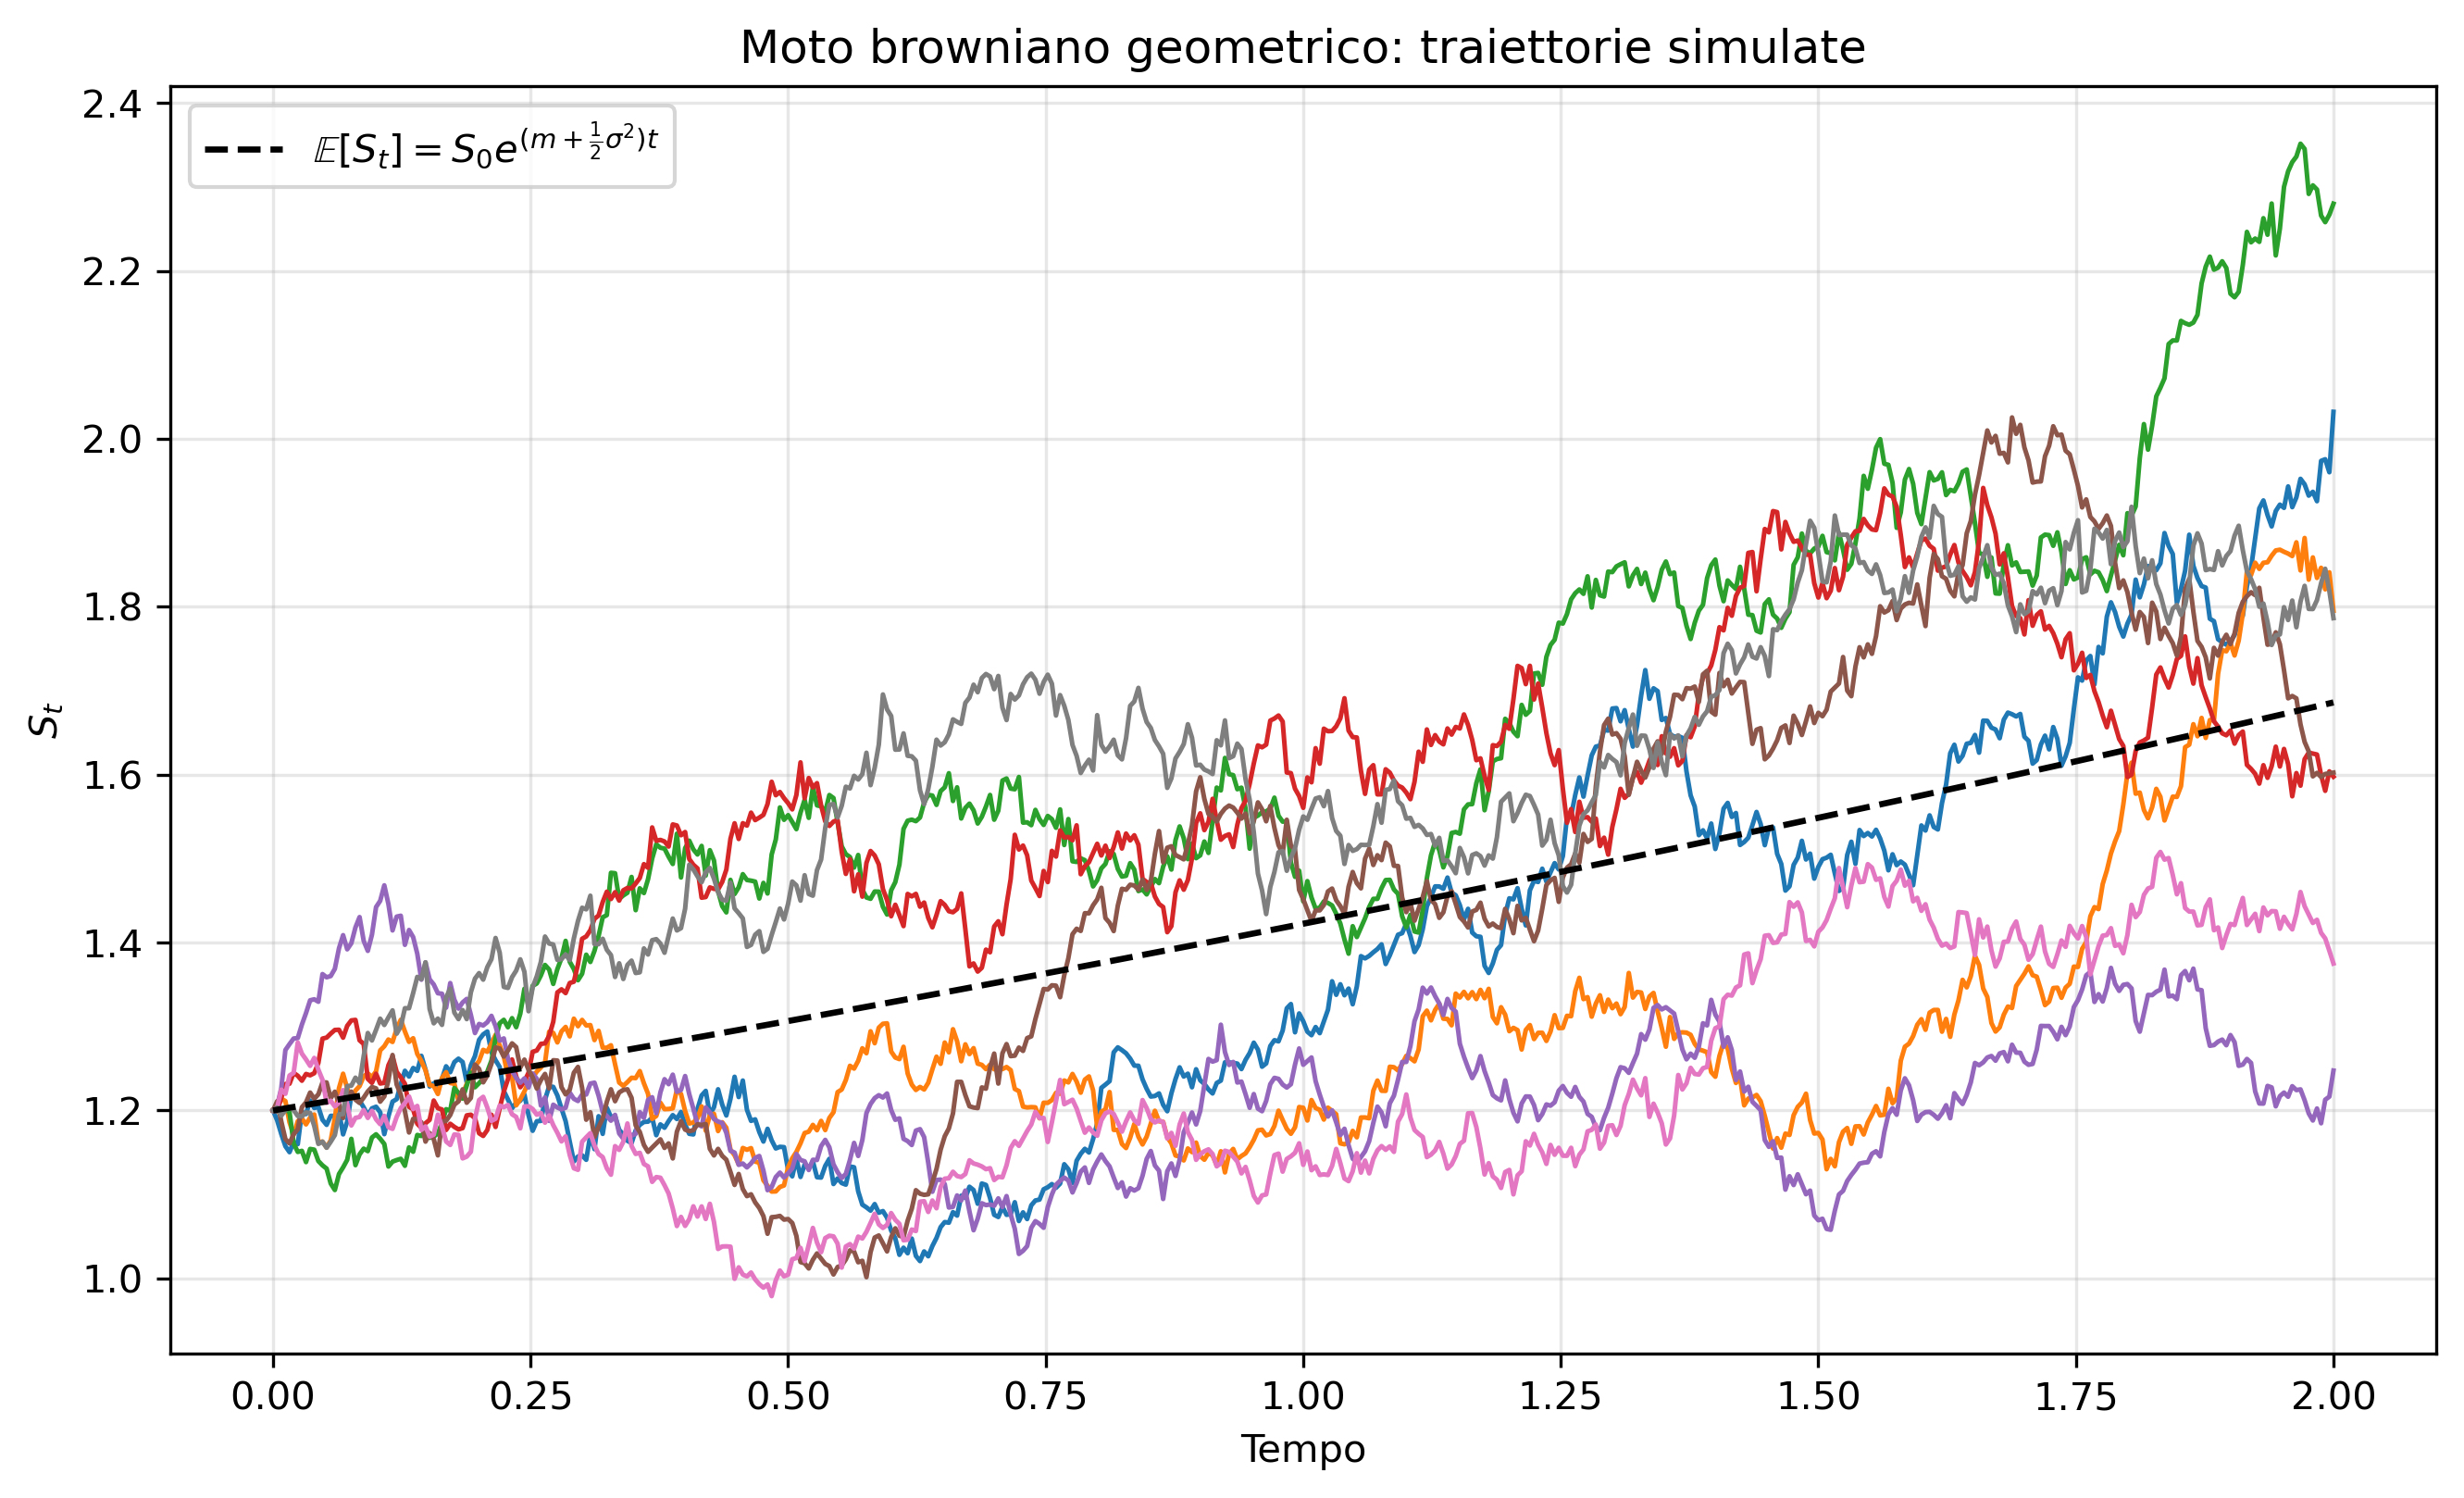
\includegraphics[width=0.68\textwidth]
{../graphics/Cap06_GBM_traiettorie.png}
\end{center}

\begin{stepitemize}

\item Un valore pi\`u elevato di $\mu$ aumenta la
\textbf{tendenza centrale di crescita} delle traiettorie.

\item Un valore pi\`u elevato di $\sigma$ aumenta la
\textbf{dispersione} delle traiettorie e dei prezzi terminali.

\end{stepitemize}
%TCIMACRO{\TeXButton{Transition: Box Out}{\transboxout}}%
%BeginExpansion
\transboxout%
%EndExpansion
%TCIMACRO{\TeXButton{EndFrame}{\end{frame}}}%
%BeginExpansion
\end{frame}%
%EndExpansion
%*

% Slide 19 - Punti di forza e limiti

%TCIMACRO{\TeXButton{BeginFrame}{\begin{frame}}}%
%BeginExpansion
\begin{frame}%
%EndExpansion

\QTR{frametitle}{Che cosa descrive bene il GBM, e che cosa no}

%TCIMACRO{\TeXButton{Transparency}{\setbeamercovered{transparent=20}}}%
%BeginExpansion
\setbeamercovered{transparent=20}%
%EndExpansion

\begin{columns}[T]

\begin{column}{0.47\textwidth}

\textbf{Punti di forza}

\begin{itemize}

\item garantisce la \textbf{positivit\`a} del prezzo;

\item rappresenta shock proporzionali al
\textbf{livello corrente};

\item produce una distribuzione esplicita e facilmente utilizzabile
nel pricing.

\end{itemize}

\end{column}

\begin{column}{0.47\textwidth}

\textbf{Limiti}

\begin{itemize}

\item assume \textbf{volatilit\`a costante};

\item non introduce alcuna
\textbf{mean reversion};

\item genera rendimenti logaritmici gaussiani e quindi
\textbf{code relativamente sottili}.

\end{itemize}

\end{column}

\end{columns}

\bigskip

Il GBM \`e il \textbf{modello di riferimento} per il Caso A.

\medskip

\textcolor{light-blue}{Per il Caso B il limite decisivo \`e l'assenza di mean reversion: un tasso o un tasso di inflazione non crescono indefinitamente come un prezzo.}
%TCIMACRO{\TeXButton{Transition: Box Out}{\transboxout}}%
%BeginExpansion
\transboxout%
%EndExpansion
%TCIMACRO{\TeXButton{EndFrame}{\end{frame}}}%
%BeginExpansion
\end{frame}%
%EndExpansion
%*

%********************
% GRUPPO 6 -  PRIMOPUNTO DI ARRIVO 
% Slide 20
% Tempo parziale: 3 minuti | Tempo cumulato: 55 minuti
% PAUSA
%********************

% Slide 20 - Punto di arrivo 

\subsection{Primo punto di arrivo}

%TCIMACRO{\TeXButton{BeginFrame}{\begin{frame}}}%
%BeginExpansion
\begin{frame}%
%EndExpansion

\QTR{frametitle}{Primo punto di arrivo}

%TCIMACRO{\TeXButton{Transparency}{\setbeamercovered{transparent=20}}}%
%BeginExpansion
\setbeamercovered{transparent=20}%
%EndExpansion

\begin{stepitemize}

\item \textbf{Passo 1 completato.} Lo shock browniano su $\Delta t$ \`e
$\sqrt{\Delta t}\,Z$: il rischio cresce con la radice dell'orizzonte.

\item \textbf{Passo 2 avviato.} Drift e diffusione rispondono alle tre
domande di progetto; il GBM compila la prima riga della scheda:

\end{stepitemize}

\begin{center}
\fbox{\parbox{0.94\textwidth}{
\scriptsize
\textbf{Requisiti (1/3)}

\smallskip

\renewcommand{\arraystretch}{1.25}
\setlength{\tabcolsep}{4pt}
\begin{tabular}{|p{0.95cm}|p{1.85cm}|p{1.55cm}|p{2.1cm}|p{2.2cm}|}
\hline
\textbf{Modello} & \textbf{Positivo?} & \textbf{Richiamo?} & \textbf{Vol. dal livello?} & \textbf{Applicazione} \\
\hline
GBM & s\`i, $S_t>0$ & no & s\`i, $\sigma S_t$ & prezzo (Caso A) \\
\hline
OU & ? & ? & ? & \\
\hline
CIR & ? & ? & ? & \\
\hline
\end{tabular}
}}
\end{center}

\medskip

\begin{center}
\textcolor{light-blue}{Caso B: quale modello per un fattore
che oscilla attorno a un livello?}
\end{center}
%TCIMACRO{\TeXButton{Transition: Box Out}{\transboxout}}%
%BeginExpansion
\transboxout%
%EndExpansion
%TCIMACRO{\TeXButton{EndFrame}{\end{frame}}}%
%BeginExpansion
\end{frame}%
%EndExpansion
%*

%********************
% GRUPPO 7 - PASSO 2b: PROCESSI MEAN-REVERTING OU E CIR (CASO B)
% Slide 21-26
% Tempo parziale: 18 minuti | Tempo cumulato seconda parte: 18 minuti
%********************

\subsection{Ornstein-Uhlenbeck}

% Slide 21 - Ornstein-Uhlenbeck: il drift di richiamo

%TCIMACRO{\TeXButton{BeginFrame}{\begin{frame}}}%
%BeginExpansion
\begin{frame}%
%EndExpansion

\QTR{frametitle}{Caso B: un drift di richiamo (Ornstein-Uhlenbeck)}

%TCIMACRO{\TeXButton{Transparency}{\setbeamercovered{transparent=20}}}%
%BeginExpansion
\setbeamercovered{transparent=20}%
%EndExpansion

\textcolor{light-blue}{Il GBM non \`e soggetto a richiamo verso una media storica. Viceversa l'inflazione oscilla attorno a un livello di lungo periodo: serve un drift che la richiami verso di esso.}

\medskip

Il processo di \textbf{Ornstein-Uhlenbeck} \`e definito da
\[
dX_t
=
\kappa(\theta-X_t)\,dt+\sigma\,dW_t,
\qquad
\kappa>0.
\]

\begin{stepitemize}

\item $\theta$ \`e il \textbf{livello di lungo periodo};
$\kappa$ misura la \textbf{velocit\`a di richiamo}.

\item Se $X_t<\theta$, allora $\kappa(\theta-X_t)>0$: il drift spinge
verso l'alto.

\item Se $X_t>\theta$, allora $\kappa(\theta-X_t)<0$: il drift spinge
verso il basso.

\end{stepitemize}

\medskip

Il processo ammette la \textbf{soluzione esplicita}
\[
X_t
=
\theta+(X_0-\theta)e^{-\kappa t}
+
\sigma \int_{0}^{t} e^{-\kappa(t-s)}\,dW_s.
\]
%TCIMACRO{\TeXButton{Transition: Box Out}{\transboxout}}%
%BeginExpansion
\transboxout%
%EndExpansion
%TCIMACRO{\TeXButton{EndFrame}{\end{frame}}}%
%BeginExpansion
\end{frame}%
%EndExpansion
%*

% Slide 22 - Media e dispersione dell'OU

%TCIMACRO{\TeXButton{BeginFrame}{\begin{frame}}}%
%BeginExpansion
\begin{frame}%
%EndExpansion

\QTR{frametitle}{L'OU: la media converge a $\theta$, la varianza si stabilizza}

%TCIMACRO{\TeXButton{Transparency}{\setbeamercovered{transparent=20}}}%
%BeginExpansion
\setbeamercovered{transparent=20}%
%EndExpansion

\begin{center}
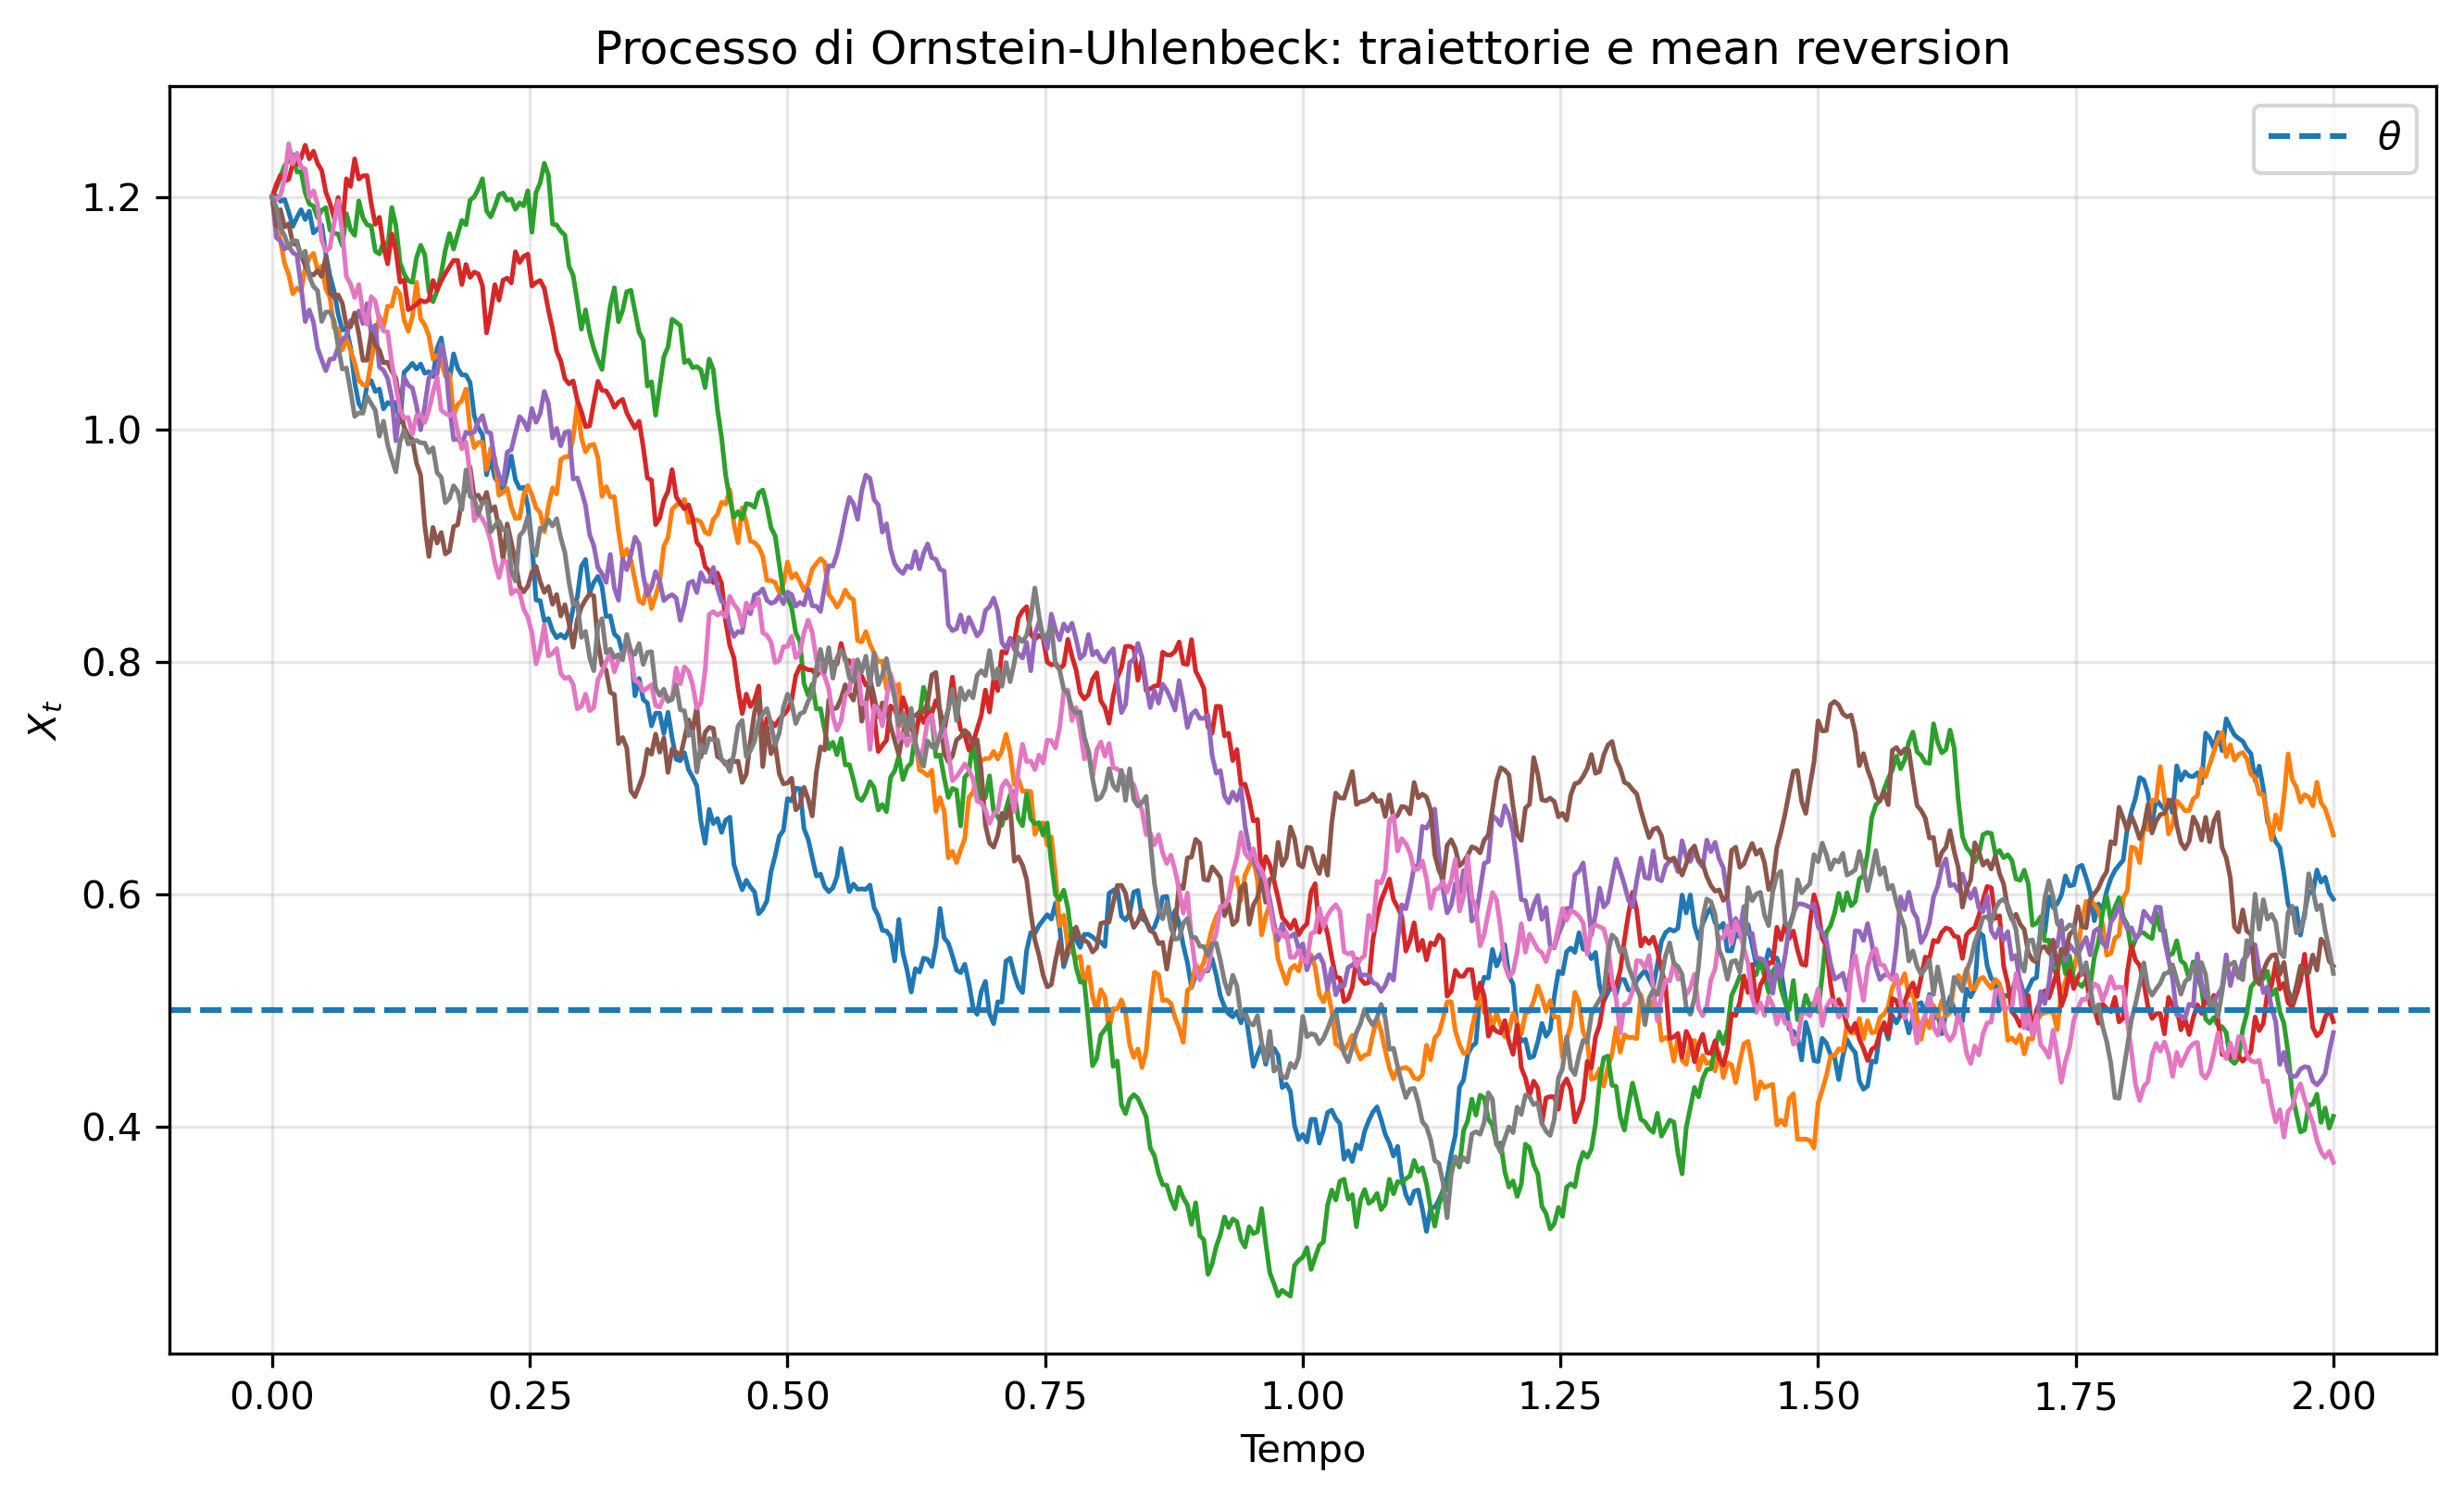
\includegraphics[width=0.56\textwidth]
{../graphics/Cap06_OU_mean_reversion.png}
\end{center}

\[
\E[X_t]
=
\theta+(X_0-\theta)e^{-\kappa t},
\qquad
\Var(X_t)
=
\frac{\sigma^2}{2\kappa}
\left(1-e^{-2\kappa t}\right).
\]

\begin{stepitemize}

\item La media converge al livello $\theta$, con velocit\`a governata
da $\kappa$.

\item La varianza non cresce indefinitamente come nel moto browniano:
converge a $\sigma^2/(2\kappa)$.

\end{stepitemize}
%TCIMACRO{\TeXButton{Transition: Box Out}{\transboxout}}%
%BeginExpansion
\transboxout%
%EndExpansion
%TCIMACRO{\TeXButton{EndFrame}{\end{frame}}}%
%BeginExpansion
\end{frame}%
%EndExpansion
%*

% Slide 23 - Requisiti (2/3) e ponte verso il CIR

%TCIMACRO{\TeXButton{BeginFrame}{\begin{frame}}}%
%BeginExpansion
\begin{frame}%
%EndExpansion

\QTR{frametitle}{Che cosa risolve l'OU, e che cosa no}

%TCIMACRO{\TeXButton{Transparency}{\setbeamercovered{transparent=20}}}%
%BeginExpansion
\setbeamercovered{transparent=20}%
%EndExpansion

\begin{center}
\fbox{\parbox{0.94\textwidth}{
\scriptsize
\textbf{Requisiti (2/3)}

\smallskip

\renewcommand{\arraystretch}{1.25}
\setlength{\tabcolsep}{4pt}
\begin{tabular}{|p{0.95cm}|p{1.85cm}|p{1.55cm}|p{2.1cm}|p{2.2cm}|}
\hline
\textbf{Modello} & \textbf{Positivo?} & \textbf{Richiamo?} & \textbf{Vol. dal livello?} & \textbf{Applicazione} \\
\hline
GBM & s\`i, $S_t>0$ & no & s\`i, $\sigma S_t$ & prezzo (Caso A) \\
\hline
OU & no, supporto $\R$ & s\`i, verso $\theta$ & no, $\sigma$ & inflazione (Caso B) \\
\hline
CIR & ? & ? & ? & \\
\hline
\end{tabular}
}}
\end{center}

\medskip

\begin{stepitemize}

\item L'OU \`e \textbf{gaussiano}: pu\`o assumere anche valori negativi.

\item Per l'inflazione del Caso B, o per uno spread, questo \`e
accettabile: anche l'inflazione pu\`o essere negativa.

\item Per il tasso $r_t$ del Caso B, o per un'intensit\`a di default,
non lo \`e: serve un richiamo che preservi la
\textbf{non negativit\`a}.

\end{stepitemize}
%TCIMACRO{\TeXButton{Transition: Box Out}{\transboxout}}%
%BeginExpansion
\transboxout%
%EndExpansion
%TCIMACRO{\TeXButton{EndFrame}{\end{frame}}}%
%BeginExpansion
\end{frame}%
%EndExpansion
%*

\subsection{Cox-Ingersoll-Ross}

% Slide 24 - CIR

%TCIMACRO{\TeXButton{BeginFrame}{\begin{frame}}}%
%BeginExpansion
\begin{frame}%
%EndExpansion

\QTR{frametitle}{CIR: stesso richiamo, diffusione che si spegne vicino a zero}

%TCIMACRO{\TeXButton{Transparency}{\setbeamercovered{transparent=20}}}%
%BeginExpansion
\setbeamercovered{transparent=20}%
%EndExpansion

Il processo \textbf{Cox-Ingersoll-Ross} \`e definito da
\[
dr_t
=
\kappa(\theta-r_t)\,dt
+
\sigma\sqrt{r_t}\,dW_t,
\qquad
r_0>0.
\]

\begin{stepitemize}

\item Il drift $\kappa(\theta-r_t)$ \`e lo stesso dell'OU: la
\textbf{mean reversion} resta.

\item Cambia la diffusione: $\sigma\sqrt{r_t}$ dipende dal
\textbf{livello corrente}.

\item Quando $r_t$ \`e vicino a zero, lo shock casuale si riduce e
prevale il richiamo verso $\theta>0$.

\item Il modello \`e adatto a grandezze \textbf{non negative}:
tassi, intensit\`a, varianze istantanee.

\item Il modello CIR \textbf{non ha una soluzione} esplicita come quelle del GBM e dell’OU: per simulare le traiettorie si discretizza.

\end{stepitemize}
%TCIMACRO{\TeXButton{Transition: Box Out}{\transboxout}}%
%BeginExpansion
\transboxout%
%EndExpansion
%TCIMACRO{\TeXButton{EndFrame}{\end{frame}}}%
%BeginExpansion
\end{frame}%
%EndExpansion
%*

% Slide 25 - Condizione di Feller

%TCIMACRO{\TeXButton{BeginFrame}{\begin{frame}}}%
%BeginExpansion
\begin{frame}%
%EndExpansion

\QTR{frametitle}{Condizione di Feller: quando il richiamo prevale sullo shock}

%TCIMACRO{\TeXButton{Transparency}{\setbeamercovered{transparent=20}}}%
%BeginExpansion
\setbeamercovered{transparent=20}%
%EndExpansion

Per il processo CIR, la \textbf{condizione di Feller} \`e
\[
2\kappa\theta
\geq
\sigma^2.
\]

\begin{stepitemize}

\item Il termine $2\kappa\theta$ misura la forza del richiamo verso un
livello positivo.

\item Il termine $\sigma^2$ misura l'intensit\`a della componente
casuale.

\item Se la condizione \`e soddisfatta, il processo non raggiunge il
confine zero, partendo da $r_0>0$.

\item Se non \`e soddisfatta, il processo pu\`o raggiungere zero,
pur rimanendo non negativo.

\end{stepitemize}

%TCIMACRO{\TeXButton{Transition: Box Out}{\transboxout}}%
%BeginExpansion
\transboxout%
%EndExpansion
%TCIMACRO{\TeXButton{EndFrame}{\end{frame}}}%
%BeginExpansion
\end{frame}%
%EndExpansion
%*

% Slide 26 - OU o CIR: requisiti (3/3)

%TCIMACRO{\TeXButton{BeginFrame}{\begin{frame}}}%
%BeginExpansion
\begin{frame}%
%EndExpansion

\QTR{frametitle}{La scheda completa: un modello per ciascun fattore}

%TCIMACRO{\TeXButton{Transparency}{\setbeamercovered{transparent=20}}}%
%BeginExpansion
\setbeamercovered{transparent=20}%
%EndExpansion

\begin{center}
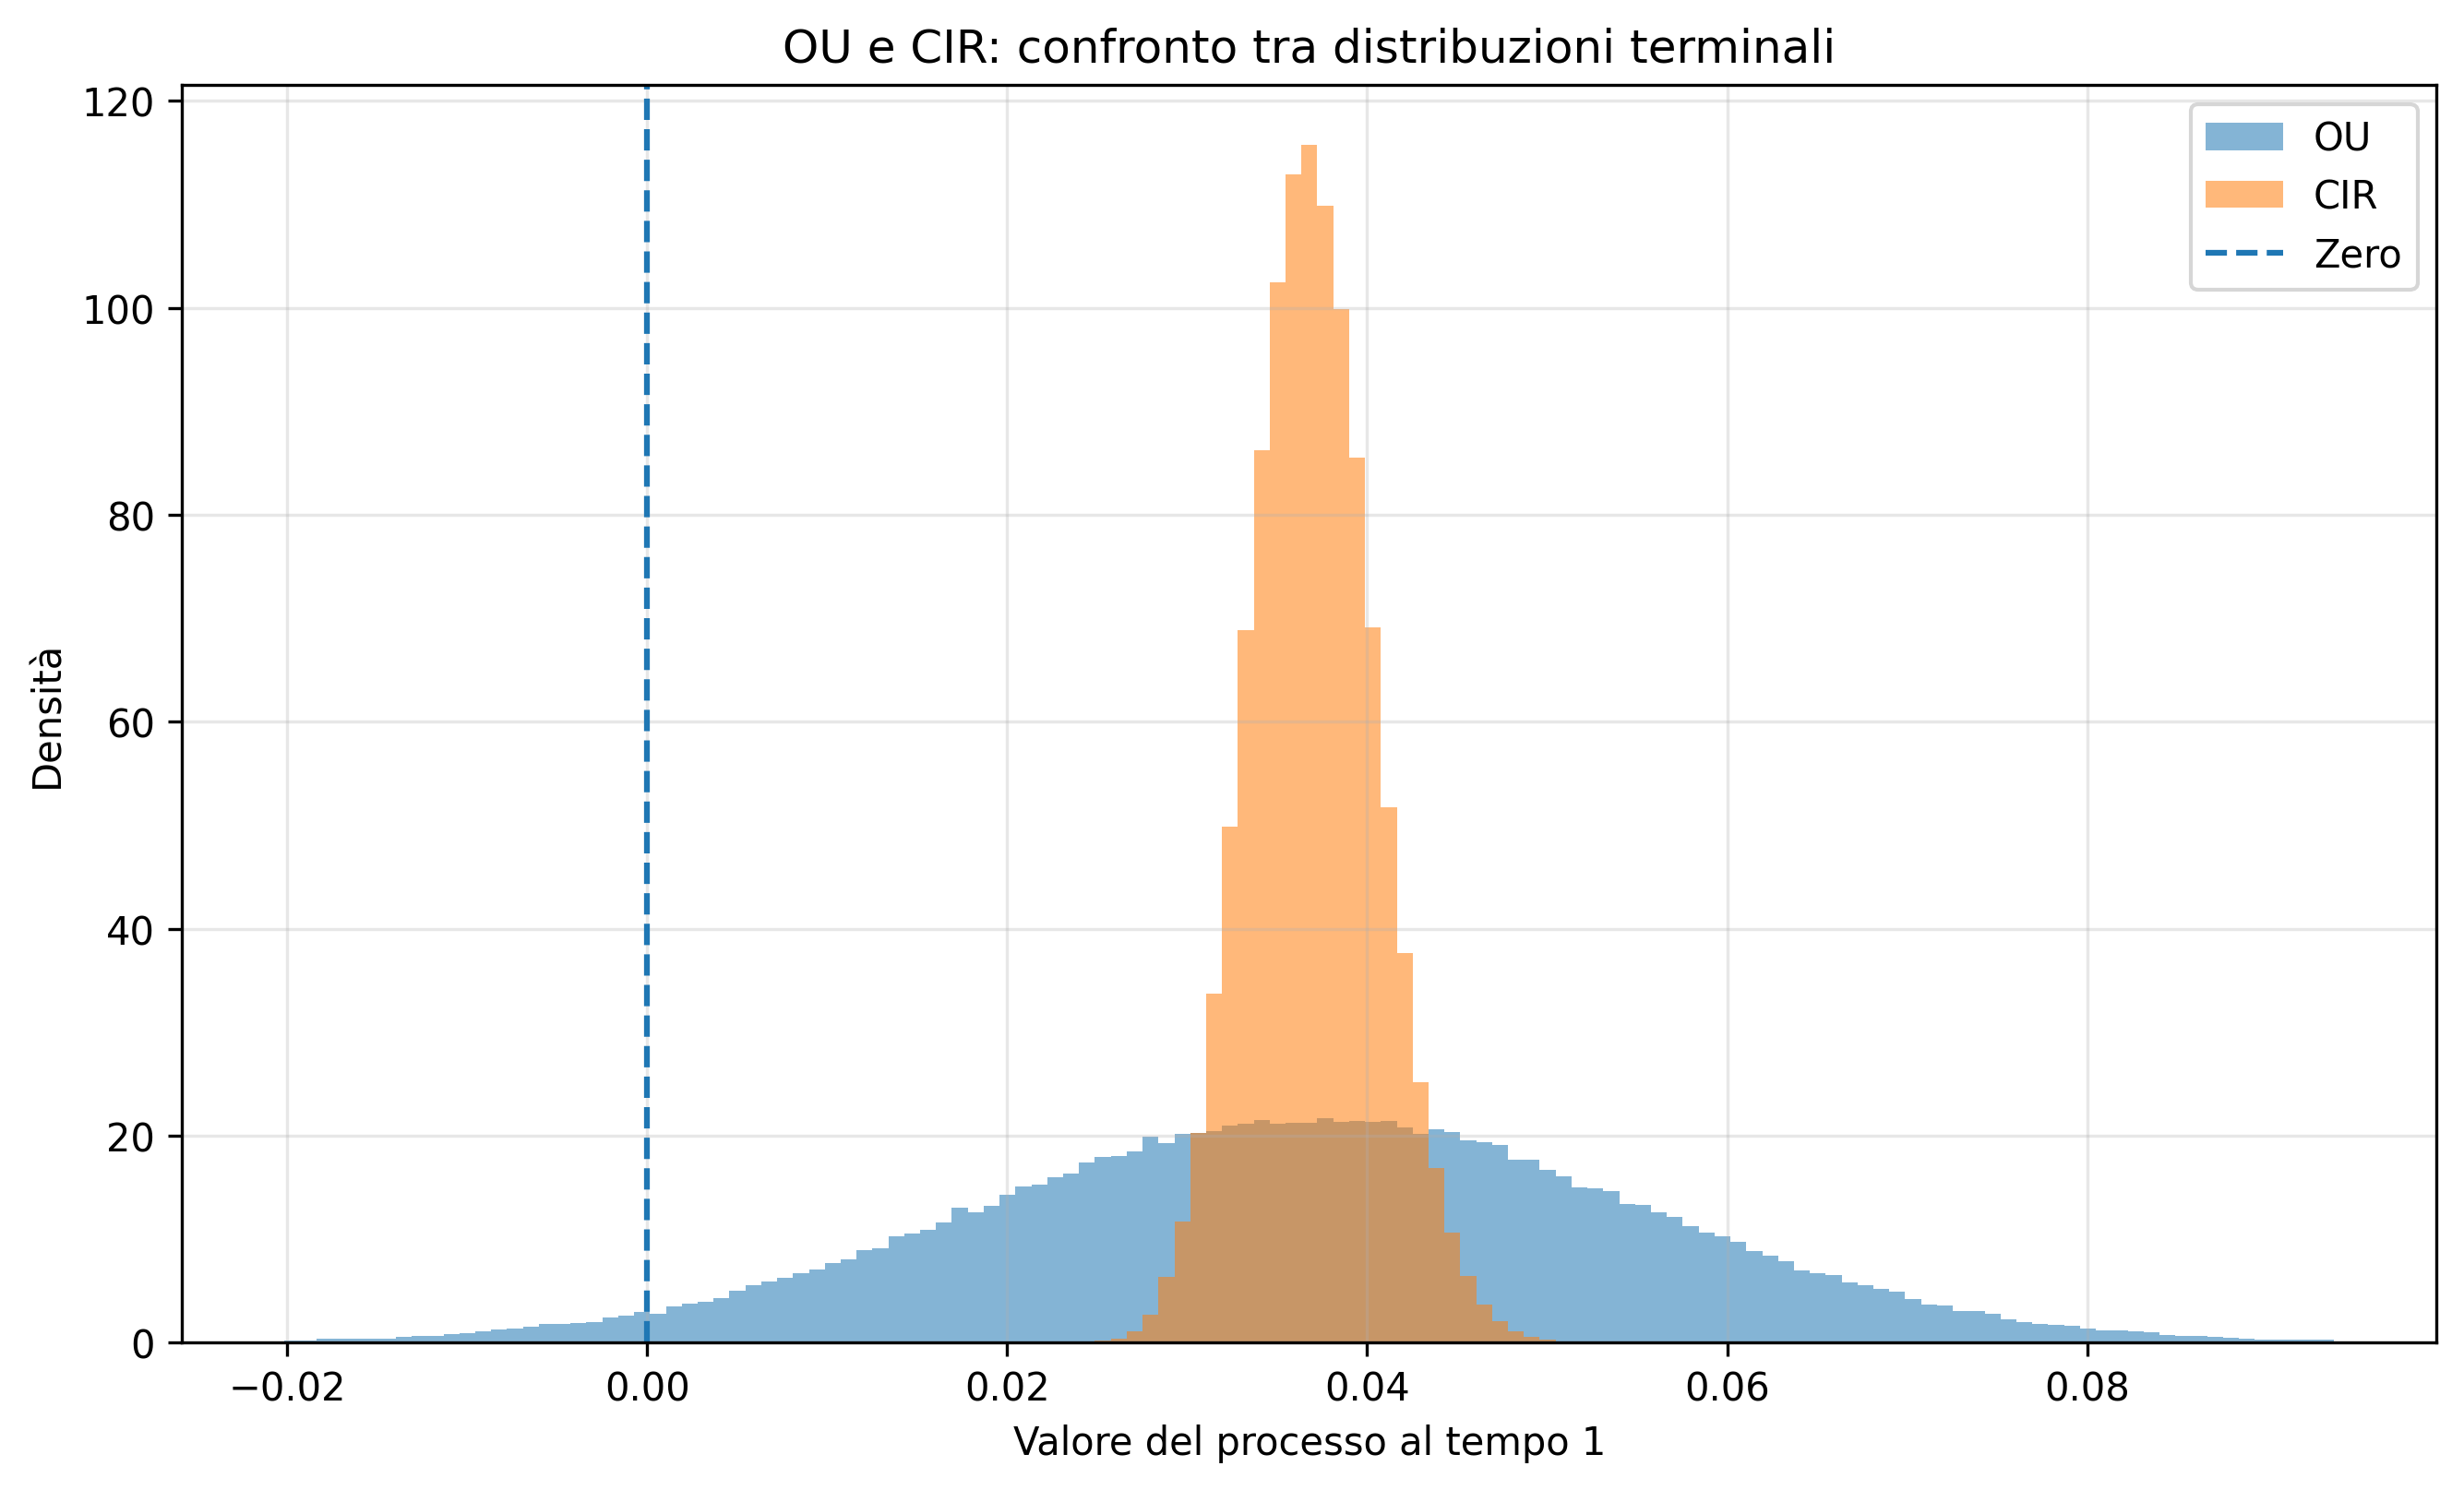
\includegraphics[width=0.46\textwidth]
{../graphics/Cap06_Es03_OU_CIR_distribuzioni_terminali.png}
\end{center}

\vspace{-0.2cm}

\begin{center}
\fbox{\parbox{0.94\textwidth}{
\scriptsize
\textbf{Requisiti (3/3)}

\smallskip

\renewcommand{\arraystretch}{1.25}
\setlength{\tabcolsep}{4pt}
\begin{tabular}{|p{0.95cm}|p{1.85cm}|p{1.55cm}|p{2.1cm}|p{2.2cm}|}
\hline
\textbf{Modello} & \textbf{Positivo?} & \textbf{Richiamo?} & \textbf{Vol. dal livello?} & \textbf{Applicazione} \\
\hline
GBM & s\`i, $S_t>0$ & no & s\`i, $\sigma S_t$ & prezzo (Caso A) \\
\hline
OU & no, supporto $\R$ & s\`i, verso $\theta$ & no, $\sigma$ & inflazione (Caso B) \\
\hline
CIR & non negativo & s\`i, verso $\theta$ & s\`i, $\sigma\sqrt{r_t}$ & tasso $r_t$ (Caso B) \\
\hline
\end{tabular}
}}
\end{center}

\smallskip

{\small Le distribuzioni terminali mostrano la differenza: l'OU ha supporto
$\R$, il CIR resta sul semiasse non negativo.}
%TCIMACRO{\TeXButton{Transition: Box Out}{\transboxout}}%
%BeginExpansion
\transboxout%
%EndExpansion
%TCIMACRO{\TeXButton{EndFrame}{\end{frame}}}%
%BeginExpansion
\end{frame}%
%EndExpansion
%*

%********************
% GRUPPO 8 - ESERCIZIO IN AULA: SCELTA DEL MODELLO E FELLER
% Slide 27-28
% Tempo parziale: 7 minuti | Tempo cumulato seconda parte: 25 minuti
%********************

% Slide 27 - Esercizio

\subsection{Esercizio: scelta tra OU e CIR}

%TCIMACRO{\TeXButton{BeginFrame}{\begin{frame}}}%
%BeginExpansion
\begin{frame}%
%EndExpansion

\QTR{frametitle}{Esercizio: quale modello per quale fattore?}

%TCIMACRO{\TeXButton{Transparency}{\setbeamercovered{transparent=20}}}%
%BeginExpansion
\setbeamercovered{transparent=20}%
%EndExpansion

\textcolor{light-blue}{La scheda dei requisiti serve anche per fattori diversi da quelli dei due casi.}

\medskip

Si considerino due fattori finanziari.

\begin{stepenumerate}

\item[1.] Uno \textbf{spread} rispetto a un valore di riferimento,
che pu\`o assumere valori sia positivi sia negativi.

\item[2.] Un'\textbf{intensit\`a di default}, che si vuole mantenere
non negativa e richiamata verso un livello di lungo periodo.

\end{stepenumerate}

\medskip

Per ciascun fattore:

\begin{itemize}

\item scegliere tra modello \textbf{OU} e modello \textbf{CIR};

\item motivare la scelta considerando \textbf{supporto} e
\textbf{diffusione}.

\end{itemize}

\medskip

Per il modello CIR si assumano inoltre
\[
\kappa=0.80,
\qquad
\theta=0.04,
\qquad
\sigma=0.20,
\]
e si verifichi se la \textbf{condizione di Feller} \`e soddisfatta.
%TCIMACRO{\TeXButton{Transition: Box Out}{\transboxout}}%
%BeginExpansion
\transboxout%
%EndExpansion
%TCIMACRO{\TeXButton{EndFrame}{\end{frame}}}%
%BeginExpansion
\end{frame}%
%EndExpansion
%*

% Slide 28 - Soluzione

\subsection{Soluzione e interpretazione}

%TCIMACRO{\TeXButton{BeginFrame}{\begin{frame}}}%
%BeginExpansion
\begin{frame}%
%EndExpansion

\QTR{frametitle}{Soluzione: spread con OU, intensit\`a con CIR}

%TCIMACRO{\TeXButton{Transparency}{\setbeamercovered{transparent=20}}}%
%BeginExpansion
\setbeamercovered{transparent=20}%
%EndExpansion

\begin{stepitemize}

\item Per lo \textbf{spread} scegliamo il modello OU:
\[
dX_t=\kappa(\theta-X_t)\,dt+\sigma\,dW_t.
\]
Il supporto \`e $\R$ e sono quindi ammessi valori negativi.

\item Per l'\textbf{intensit\`a di default} scegliamo il modello CIR:
\[
dr_t=\kappa(\theta-r_t)\,dt+\sigma\sqrt{r_t}\,dW_t.
\]
La diffusione si riduce quando $r_t$ si avvicina a zero.

\end{stepitemize}

Per la condizione di Feller:
\[
2\kappa\theta
=
2(0.80)(0.04)
=
0.064,
\qquad
\sigma^2
=
0.20^2
=
0.040.
\]
Poich\'e $2\kappa\theta>\sigma^2$, la condizione \`e soddisfatta:
partendo da un valore positivo, il processo CIR \textbf{non raggiunge il
confine zero}.
%TCIMACRO{\TeXButton{Transition: Box Out}{\transboxout}}%
%BeginExpansion
\transboxout%
%EndExpansion
%TCIMACRO{\TeXButton{EndFrame}{\end{frame}}}%
%BeginExpansion
\end{frame}%
%EndExpansion
%*

%********************
% GRUPPO 9 - PASSO 3: LA DIPENDENZA (SHOCK CORRELATI)
% Divisorio + Slide 29-31
% Tempo parziale: 11 minuti | Tempo cumulato seconda parte: 36 minuti
%********************

\section{\texorpdfstring{Passo 3 -- La dipendenza}{Passo 3 - La dipendenza}}

%TCIMACRO{\TeXButton{BeginFrame}{\begin{frame}}}%
%BeginExpansion
\begin{frame}%
%EndExpansion

\setbeamertemplate{headline}{}

\vfill

\begin{center}
\textcolor{light-blue}{{\Large \textbf{Passo 3 -- La dipendenza: shock correlati}}}
\end{center}

\vfill

{\scriptsize
\renewcommand{\arraystretch}{1.3}
\begin{center}
\begin{tabular}{|c|p{1.9cm}|p{4.9cm}|p{2.7cm}|}
\hline
\textbf{Passo} & \textbf{Tema} & \textbf{Domanda} & \textbf{Strumento} \\
\hline
1 & Il rumore & Quanto \`e grande uno shock su $\Delta t$? & $W_t$, scala $\sqrt{\Delta t}$ \\
\hline
2 & La forma & Quali propriet\`a deve avere il fattore? & SDE: GBM, OU, CIR \\
\hline
\leavevmode\alert{3} & \leavevmode\alert{La dipendenza} & \leavevmode\alert{I fattori si muovono insieme?} & \leavevmode\alert{shock correlati} \\
\hline
4 & La simulazione & Come si genera la traiettoria? & Eulero-Maruyama \\
\hline
\end{tabular}
\end{center}
}

\vfill

%TCIMACRO{\TeXButton{Transition: Box Out}{\transboxout}}%
%BeginExpansion
\transboxout%
%EndExpansion
%TCIMACRO{\TeXButton{EndFrame}{\end{frame}}}%
%BeginExpansion
\end{frame}%
%EndExpansion
%*

% Slide 29 - Motivazione multivariata dal Caso B

\subsection{Fattori congiunti}

%TCIMACRO{\TeXButton{BeginFrame}{\begin{frame}}}%
%BeginExpansion
\begin{frame}%
%EndExpansion

\QTR{frametitle}{Caso B: inflazione e tasso non si muovono separatamente}

%TCIMACRO{\TeXButton{Transparency}{\setbeamercovered{transparent=20}}}%
%BeginExpansion
\setbeamercovered{transparent=20}%
%EndExpansion

\textcolor{light-blue}{Ora abbiamo un modello per ciascun fattore. Ma nel Caso B inflazione e tasso reagiscono agli stessi eventi macroeconomici.}

\medskip

\begin{stepitemize}

\item Simulare i due fattori con shock indipendenti significherebbe
ignorare questa dipendenza.

\item Le repliche Monte Carlo devono essere coerenti anche
nella \textbf{struttura di dipendenza} tra fattori.

\item La correlazione tra shock modifica la \textbf{diversificazione}
e quindi la distribuzione del valore della posizione.

\end{stepitemize}

\[
\text{shock indipendenti}
\longrightarrow
\text{shock correlati}
\longrightarrow
\text{fattori}
\longrightarrow
\text{rischio}.
\]

Lo stesso vale per qualunque portafoglio esposto a pi\`u fattori:
prezzi azionari, tassi, cambi, commodities.
%TCIMACRO{\TeXButton{Transition: Box Out}{\transboxout}}%
%BeginExpansion
\transboxout%
%EndExpansion
%TCIMACRO{\TeXButton{EndFrame}{\end{frame}}}%
%BeginExpansion
\end{frame}%
%EndExpansion
%*

% Slide 30 - Costruzione degli shock correlati

\subsection{Shock correlati}

%TCIMACRO{\TeXButton{BeginFrame}{\begin{frame}}}%
%BeginExpansion
\begin{frame}%
%EndExpansion

\QTR{frametitle}{Da shock indipendenti a shock correlati: decomposizione di Cholesky}

%TCIMACRO{\TeXButton{Transparency}{\setbeamercovered{transparent=20}}}%
%BeginExpansion
\setbeamercovered{transparent=20}%
%EndExpansion

Si parte da un vettore di normali standard indipendenti e si costruisce
\[
Z=
\begin{pmatrix}Z_1\\Z_2\end{pmatrix}
\sim\mathcal{N}(0,I),
\qquad
L=
\begin{pmatrix}
1 & 0\\
\rho & \sqrt{1-\rho^2}
\end{pmatrix},
\qquad
\varepsilon=LZ.
\]
\[
\varepsilon_1=Z_1,
\qquad
\varepsilon_2
=
\rho Z_1+\sqrt{1-\rho^2}\,Z_2.
\]
Allora
\[
\E[\varepsilon_1]=\E[\varepsilon_2]=0,
\qquad
\Var(\varepsilon_1)=\Var(\varepsilon_2)=1,
\qquad
\Corr(\varepsilon_1,\varepsilon_2)=\rho,
\]
cio\`e $\varepsilon$ ha matrice di correlazione
$R=LL'=\begin{pmatrix}1 & \rho\\ \rho & 1\end{pmatrix}$.

\medskip
Con $d$ fattori, $L$ si ottiene da $R$ con la decomposizione di
Cholesky. Gli incrementi browniani correlati sono
$\Delta W_t^i=\sqrt{\Delta t}\,\varepsilon_i$.
%TCIMACRO{\TeXButton{Transition: Box Out}{\transboxout}}%
%BeginExpansion
\transboxout%
%EndExpansion
%TCIMACRO{\TeXButton{EndFrame}{\end{frame}}}%
%BeginExpansion
\end{frame}%
%EndExpansion
%*

% Slide 31 - Correlazione e rischio della posizione

\subsection{Rischio di portafoglio}

%TCIMACRO{\TeXButton{BeginFrame}{\begin{frame}}}%
%BeginExpansion
\begin{frame}%
%EndExpansion

\QTR{frametitle}{La correlazione cambia il rischio della posizione}

%TCIMACRO{\TeXButton{Transparency}{\setbeamercovered{transparent=20}}}%
%BeginExpansion
\setbeamercovered{transparent=20}%
%EndExpansion

\begin{center}
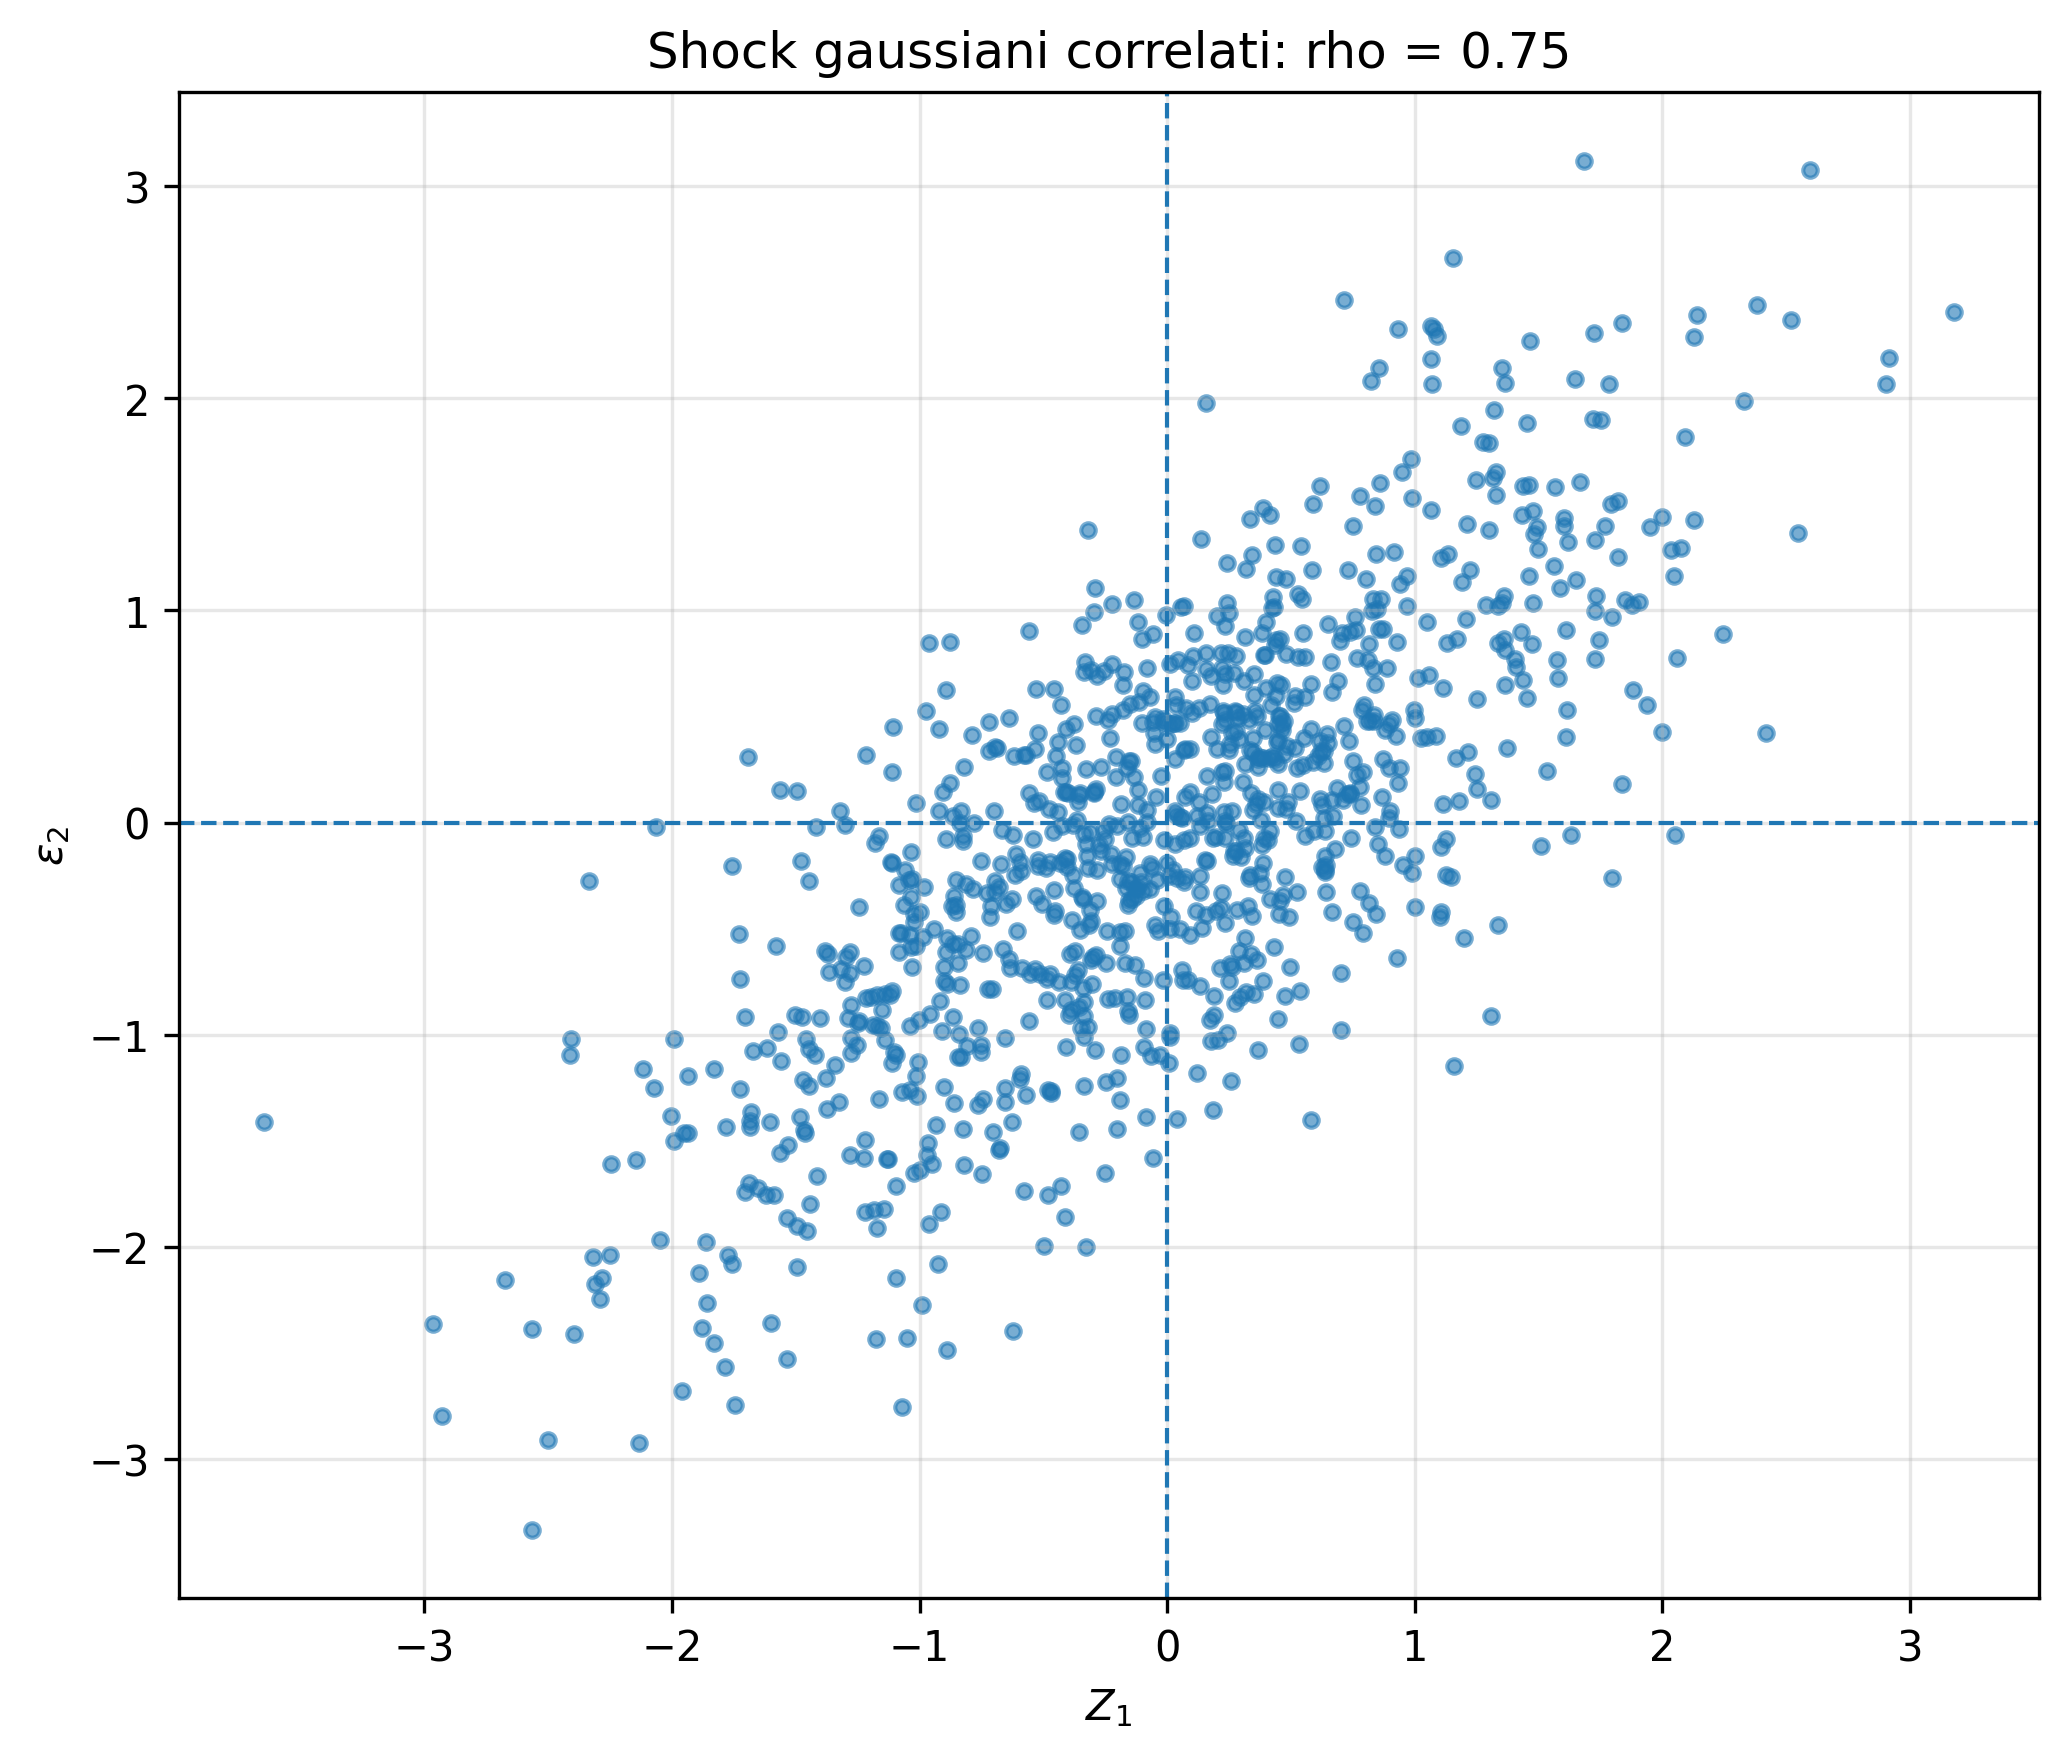
\includegraphics[width=0.34\textwidth]
{../graphics/Cap06_correlated_gaussian_shocks.png}
\end{center}

Una posizione ha esposizioni $V_1,V_2$ a due fattori con shock
$\sigma_1\Delta W_t^1$ e $\sigma_2\Delta W_t^2$, dove
$\Corr(\Delta W_t^1,\Delta W_t^2)=\rho$:
{\small
\[
\Var\left(V_1\sigma_1\Delta W_t^1+V_2\sigma_2\Delta W_t^2\right)
=
\left(V_1^2\sigma_1^2+V_2^2\sigma_2^2+2\rho V_1V_2\sigma_1\sigma_2\right)\Delta t.
\]
}

Ponendo $V_1=V_2=1$, $\sigma_1=\sigma_2=0.20$ e $\Delta t=1$, la varianza \`{e}
$0.08(1+\rho)$. Fissando $\rho=0.75$, come in figura, la varianza della posizione vale $0.14$; con shock
indipendenti vale $0.08$; con $\rho=-0.75$ vale $0.02$.
%TCIMACRO{\TeXButton{Transition: Box Out}{\transboxout}}%
%BeginExpansion
\transboxout%
%EndExpansion
%TCIMACRO{\TeXButton{EndFrame}{\end{frame}}}%
%BeginExpansion
\end{frame}%
%EndExpansion
%*


% GRUPPO 10 - PASSO 4: LA SIMULAZIONE (EULERO-MARUYAMA)
% Divisorio + Slide 32-34
% Tempo parziale: 14 minuti | Tempo cumulato seconda parte: 50 minuti
%********************

\section{\texorpdfstring{Passo 4 -- La simulazione}{Passo 4 - La simulazione}}

%TCIMACRO{\TeXButton{BeginFrame}{\begin{frame}}}%
%BeginExpansion
\begin{frame}%
%EndExpansion

\setbeamertemplate{headline}{}

\vfill

\begin{center}
\textcolor{light-blue}{{\Large \textbf{Passo 4 -- La simulazione: dalla SDE alla griglia}}}
\end{center}

\vfill

{\scriptsize
\renewcommand{\arraystretch}{1.3}
\begin{center}
\begin{tabular}{|c|p{1.9cm}|p{4.9cm}|p{2.7cm}|}
\hline
\textbf{Passo} & \textbf{Tema} & \textbf{Domanda} & \textbf{Strumento} \\
\hline
1 & Il rumore & Quanto \`e grande uno shock su $\Delta t$? & $W_t$, scala $\sqrt{\Delta t}$ \\
\hline
2 & La forma & Quali propriet\`a deve avere il fattore? & SDE: GBM, OU, CIR \\
\hline
3 & La dipendenza & I fattori si muovono insieme? & shock correlati \\
\hline
\leavevmode\alert{4} & \leavevmode\alert{La simulazione} & \leavevmode\alert{Come si genera una traiettoria?} & \leavevmode\alert{Eulero-Maruyama} \\
\hline
\end{tabular}
\end{center}
}

\vfill

%TCIMACRO{\TeXButton{Transition: Box Out}{\transboxout}}%
%BeginExpansion
\transboxout%
%EndExpansion
%TCIMACRO{\TeXButton{EndFrame}{\end{frame}}}%
%BeginExpansion
\end{frame}%
%EndExpansion
%*

% Slide 32 - Dalla SDE alla griglia temporale

\subsection{Eulero-Maruyama}

%TCIMACRO{\TeXButton{BeginFrame}{\begin{frame}}}%
%BeginExpansion
\begin{frame}%
%EndExpansion

\QTR{frametitle}{Si torna alla griglia: lo stesso $\sqrt{\Delta t}\,Z$ del passo 1}

%TCIMACRO{\TeXButton{Transparency}{\setbeamercovered{transparent=20}}}%
%BeginExpansion
\setbeamercovered{transparent=20}%
%EndExpansion

\textcolor{light-blue}{Nel passo 1 siamo partiti da una griglia per costruire $W_t$; ora torniamo sulla griglia per generare le traiettorie di $X_t$.}

\medskip

Data la SDE
\[
dX_t=a(X_t,t)\,dt+b(X_t,t)\,dW_t,
\]
lo schema di \textbf{Eulero-Maruyama} con passo $\Delta t$ \`e
\[
X_{t+\Delta t}
=
X_t
+
a(X_t,t)\Delta t
+
b(X_t,t)\sqrt{\Delta t}\,Z_{t+\Delta t},
\qquad
Z_{t+\Delta t}\sim\mathcal{N}(0,1).
\]

\begin{stepitemize}
\item Su $[t,t+\Delta t]$ drift e diffusione vengono congelati al valore
corrente $X_t$.
\item L'incremento browniano \`e sostituito dallo shock simulabile
$\sqrt{\Delta t}\,Z_{t+\Delta t}$, come nella passeggiata riscalata.
\item Con pi\`u fattori, gli shock sono le componenti di $\varepsilon=LZ$
del passo 3.
\end{stepitemize}
%TCIMACRO{\TeXButton{Transition: Box Out}{\transboxout}}%
%BeginExpansion
\transboxout%
%EndExpansion
%TCIMACRO{\TeXButton{EndFrame}{\end{frame}}}%
%BeginExpansion
\end{frame}%
%EndExpansion
%*

% Slide 33 - Un passo mensile per il GBM

\subsection{Un passo per il GBM}

%TCIMACRO{\TeXButton{BeginFrame}{\begin{frame}}}%
%BeginExpansion
\begin{frame}%
%EndExpansion

\QTR{frametitle}{Caso A: un passo mensile per il GBM}

%TCIMACRO{\TeXButton{Transparency}{\setbeamercovered{transparent=20}}}%
%BeginExpansion
\setbeamercovered{transparent=20}%
%EndExpansion

Per il GBM $dS_t=\mu S_t\,dt+\sigma S_t\,dW_t$ lo schema Eulero-Maruyama (EM) per $S_t $ offre:
\[
S_{t+\Delta t}^{\mathrm{EM}}
=
S_t^{\mathrm{EM}}
\left(
1+\mu\Delta t+\sigma\sqrt{\Delta t}\,Z_{t+\Delta t}
\right).
\]
Partendo da $t=0$, con
\[
S_0=100,\quad
\mu=0.06,\quad
\sigma=0.20,\quad
\Delta t=\frac{1}{12},\quad
Z_{\Delta t}=-1.1,
\]
lo shock browniano \`e
\[
\sqrt{\Delta t}\,Z_{\Delta t}
=
\sqrt{\frac{1}{12}}(-1.1)
\approx
-0.31754.
\]
Quindi
\[
S_{\Delta t}^{\mathrm{EM}}
=
100
\left[
1+0.06\cdot\frac{1}{12}
+0.20(-0.31754)
\right]
\approx
94.149.
\]
%TCIMACRO{\TeXButton{Transition: Box Out}{\transboxout}}%
%BeginExpansion
\transboxout%
%EndExpansion
%TCIMACRO{\TeXButton{EndFrame}{\end{frame}}}%
%BeginExpansion
\end{frame}%
%EndExpansion
%*

%********************

% Slide 34a - Errore di discretizzazione in un passo

\subsection{Errore in un passo}

%TCIMACRO{\TeXButton{BeginFrame}{\begin{frame}}}%
%BeginExpansion
\begin{frame}%
%EndExpansion

\QTR{frametitle}{Il prezzo della discretizzazione: l'errore in un passo}

%TCIMACRO{\TeXButton{Transparency}{\setbeamercovered{transparent=20}}}%
%BeginExpansion
\setbeamercovered{transparent=20}%
%EndExpansion

Con lo stesso shock $\sqrt{\Delta t}\,Z_{\Delta t}\approx-0.31754$, la
soluzione esplicita del GBM d\`{a} il valore esatto
{\small
\[
S_{\Delta t}
=
100
\exp\left\{
\left(0.06-\frac{1}{2}0.20^2\right)\frac{1}{12}
+
0.20(-0.31754)
\right\}
\approx
94.160,
\]
}
contro il valore approssimato $S_{\Delta t}^{\mathrm{EM}}\approx94.149$:
un \textbf{errore di discretizzazione} di circa $0.011$ in un solo passo.

\begin{stepitemize}
\item Lo shock \`{e} lo stesso: la differenza dipende solo dallo schema,
che congela drift e diffusione al valore iniziale del passo.
\item Su una traiettoria gli errori dei singoli passi si accumulano.
\item Le propriet\`{a} del modello continuo, ottenute con la scelta di
drift e diffusione, non passano automaticamente allo schema discreto:
con uno shock molto sfavorevole,
$1+\mu\Delta t+\sigma\sqrt{\Delta t}\,Z_{t+\Delta t}$ pu\`{o} diventare
negativo e con esso $S_{t+\Delta t}^{\mathrm{EM}}$. La
\textbf{positivit\`{a}} del GBM e la \textbf{non negativit\`{a}} del CIR
vanno controllate nella simulazione.
\end{stepitemize}
%TCIMACRO{\TeXButton{Transition: Box Out}{\transboxout}}%
%BeginExpansion
\transboxout%
%EndExpansion
%TCIMACRO{\TeXButton{EndFrame}{\end{frame}}}%
%BeginExpansion
\end{frame}%
%EndExpansion
%*

% Slide 34b - Qualita' della simulazione lungo la traiettoria

\subsection{Qualit\`{a} della simulazione}

%TCIMACRO{\TeXButton{BeginFrame}{\begin{frame}}}%
%BeginExpansion
\begin{frame}%
%EndExpansion

\QTR{frametitle}{Lungo la traiettoria: la qualit\`{a} dipende dal passo}

%TCIMACRO{\TeXButton{Transparency}{\setbeamercovered{transparent=20}}}%
%BeginExpansion
\setbeamercovered{transparent=20}%
%EndExpansion

\begin{center}
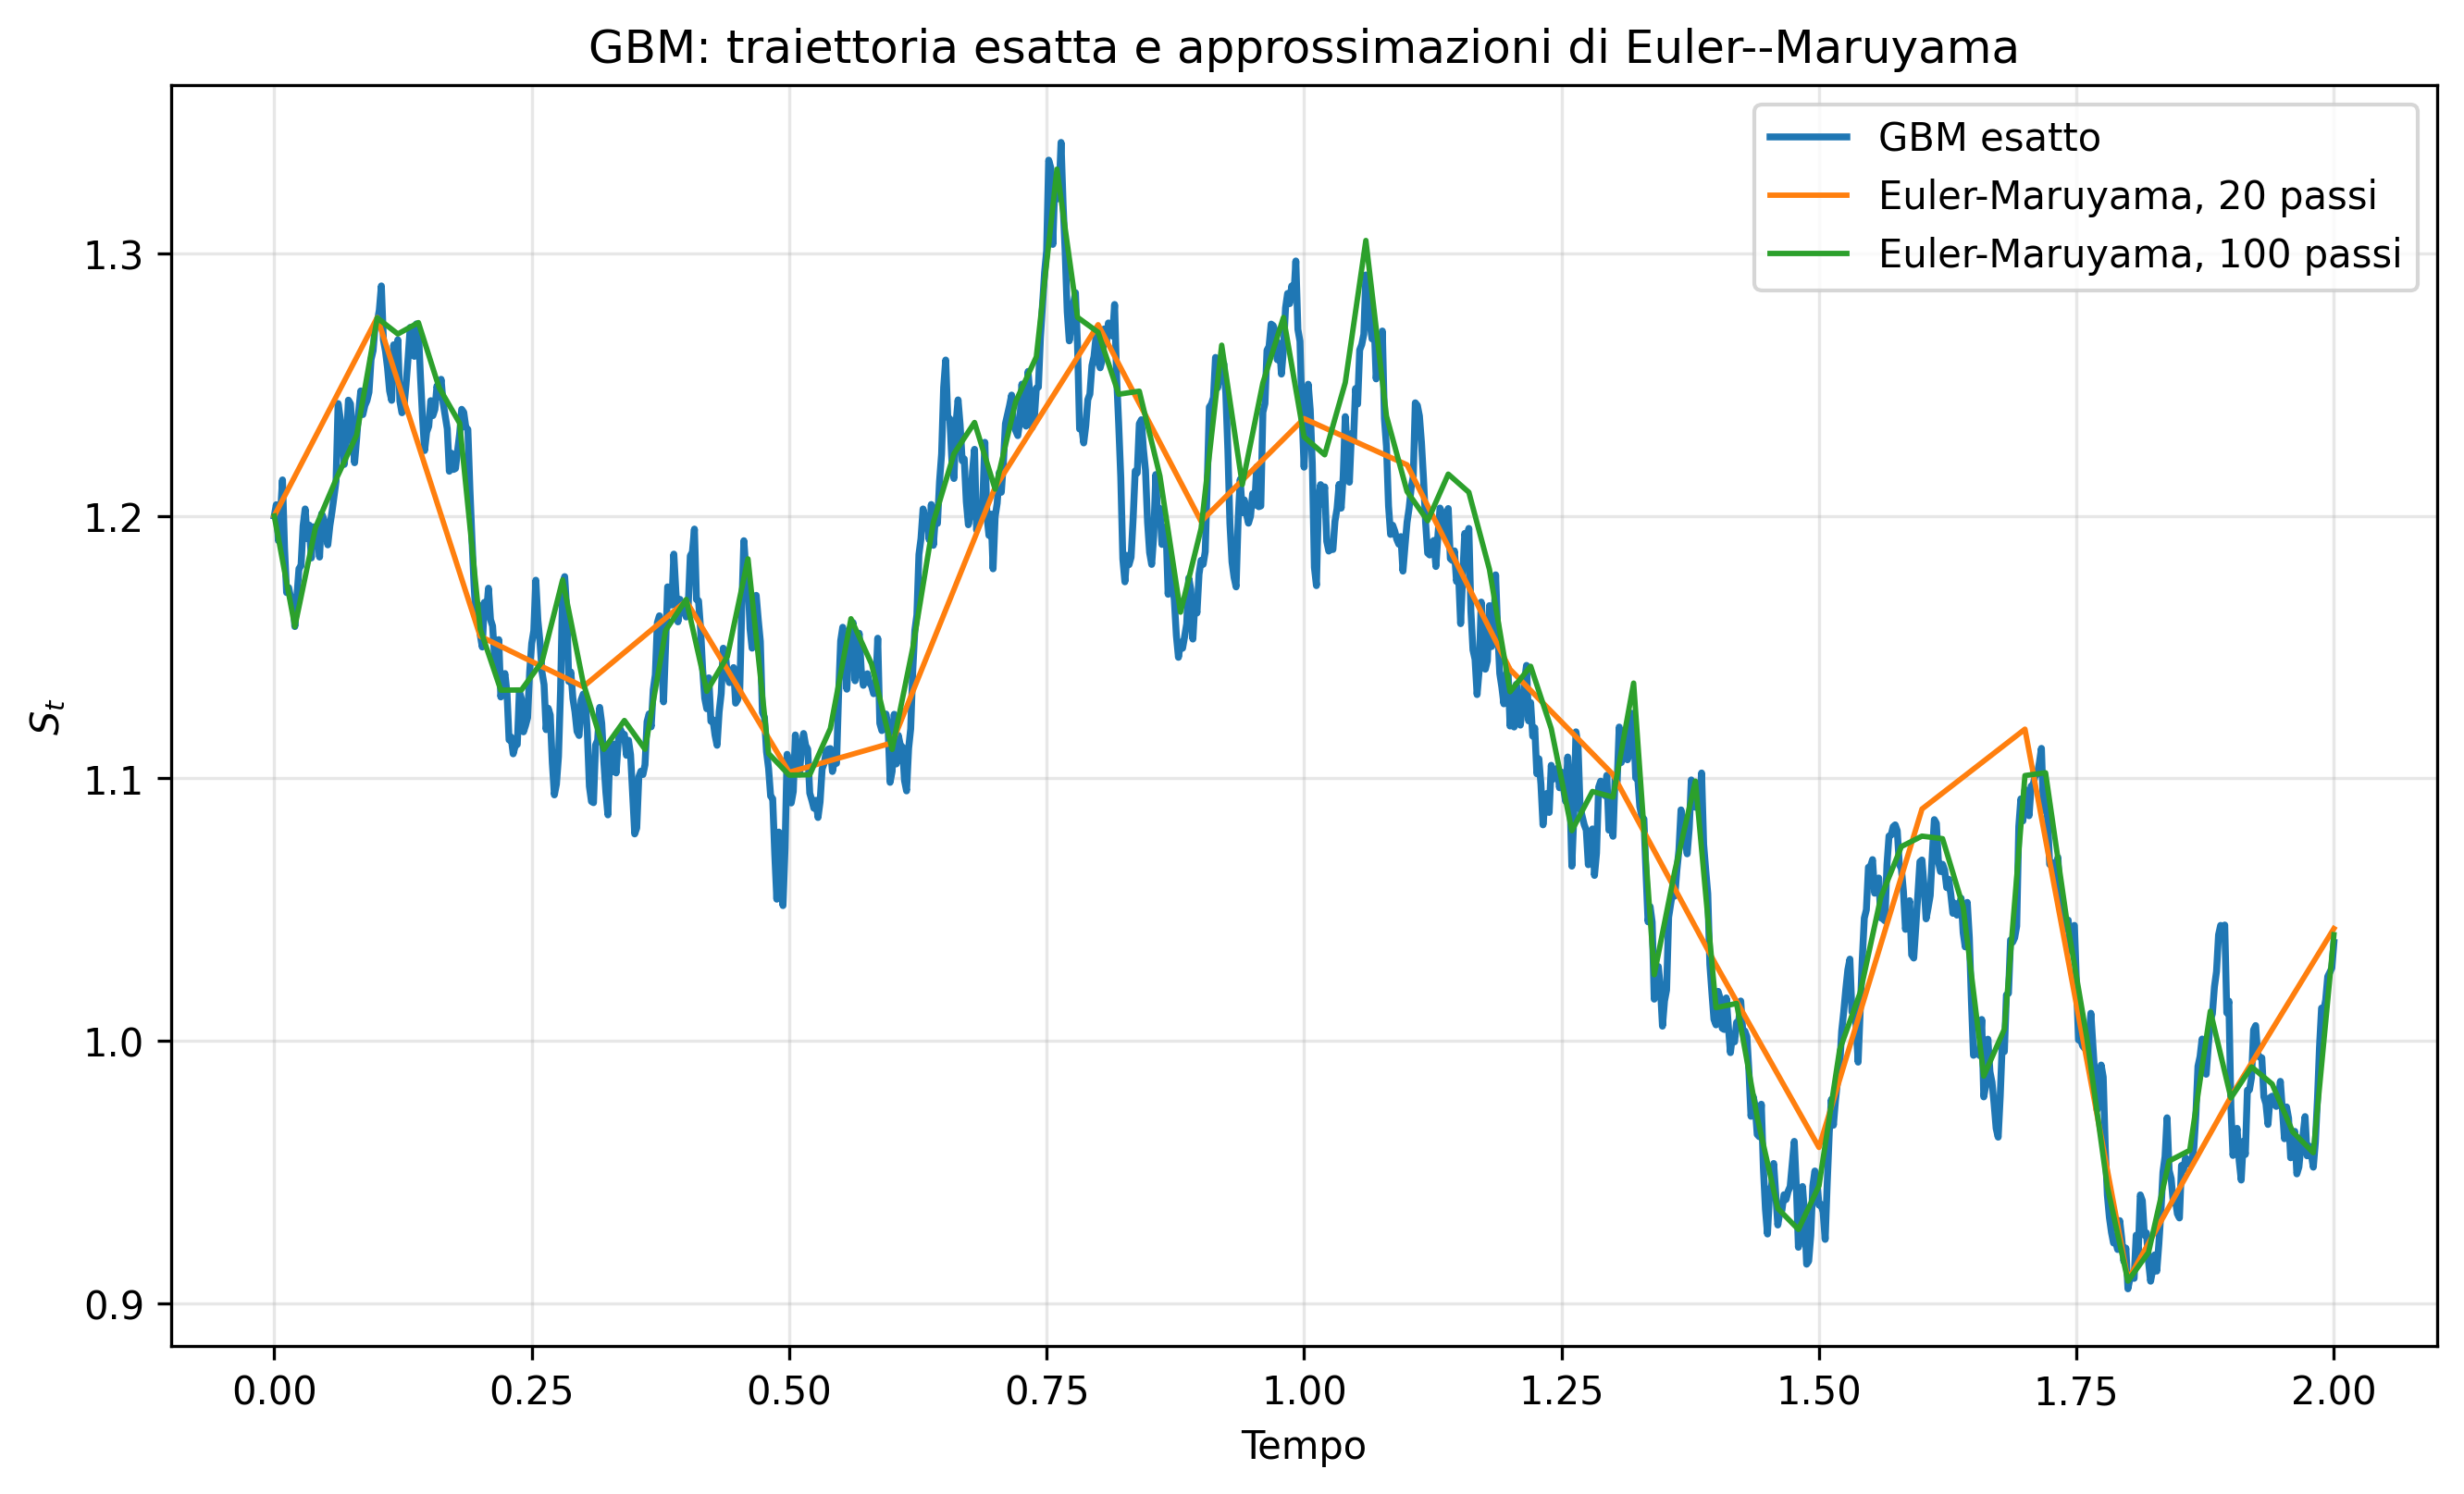
\includegraphics[width=0.8\textwidth]
{../graphics/Cap06_EulerMaruyama_GBM_confronto.png}
\end{center}

\vspace{-0.15cm}

{\small
Stessa realizzazione browniana: con $20$ passi ($\Delta t=0.1$) lo schema
perde le oscillazioni interne al passo; con $100$ passi ($\Delta t=0.02$)
segue da vicino la traiettoria esatta. Griglia pi\`{u} fine: errore
minore, \textbf{costo computazionale} maggiore.
}
%TCIMACRO{\TeXButton{Transition: Box Out}{\transboxout}}%
%BeginExpansion
\transboxout%
%EndExpansion
%TCIMACRO{\TeXButton{EndFrame}{\end{frame}}}%
%BeginExpansion
\end{frame}%
%EndExpansion
%*


%********************
% GRUPPO 11 - SINTESI E RACCORDO CON PYTHON
% Slide 35
% Tempo parziale: 5 minuti | Tempo cumulato seconda parte: 55 minuti
%********************

\section{Sintesi}

% Sintesi e raccordo con Python

\subsection{Raccordo con Python}

%TCIMACRO{\TeXButton{BeginFrame}{\begin{frame}}}%
%BeginExpansion
\begin{frame}%
%EndExpansion

\QTR{frametitle}{Sintesi: dal rumore alle traiettorie dei due casi}

%TCIMACRO{\TeXButton{Transparency}{\setbeamercovered{transparent=20}}}%
%BeginExpansion
\setbeamercovered{transparent=20}%
%EndExpansion

{\scriptsize
\renewcommand{\arraystretch}{1.3}
\begin{center}
\begin{tabular}{|c|p{1.9cm}|p{6.6cm}|}
\hline
\textbf{Passo} & \textbf{Tema} & \textbf{Risultato} \\
\hline
1 & Il rumore & $\Delta W_t=\sqrt{\Delta t}\,Z$: il rischio cresce con $\sqrt{h}$ \\
\hline
2 & La forma & drift e diffusione scelti dai requisiti: GBM, OU, CIR \\
\hline
3 & La dipendenza & shock correlati $\varepsilon=LZ$, con $R=LL'$ \\
\hline
4 & La simulazione & Eulero-Maruyama: traiettorie su griglia, con errore da controllare \\
\hline
\end{tabular}
\end{center}
}

\begin{stepitemize}
\item \textbf{Caso A.} Il prezzo $S_t$ segue un GBM; le traiettorie
simulate alimentano la valutazione del contratto sulla media dei prezzi.
\item \textbf{Caso B.} L'inflazione segue un OU, il tasso $r_t$ un CIR,
con shock correlati; le traiettorie alimentano la valutazione
dell'obbligazione indicizzata.
\end{stepitemize}

\medskip

La Lezione 7 traduce questo percorso in procedure Python:
\[
\begin{gathered}
\text{modello continuo}
\longrightarrow
\text{discretizzazione}
\longrightarrow
\text{traiettorie simulate}
\\
\longrightarrow
\text{pricing e rischio}.
\end{gathered}
\]
%TCIMACRO{\TeXButton{Transition: Box Out}{\transboxout}}%
%BeginExpansion
\transboxout%
%EndExpansion
%TCIMACRO{\TeXButton{EndFrame}{\end{frame}}}%
%BeginExpansion
\end{frame}%
%EndExpansion
%*

\end{document}
